\documentclass[12pt, a4paper, tocpage=plain]{abnt} % Fonte tamanho 12, papel A4, páginas do sumário sem o p.<número da página>

\usepackage[brazilian]{babel} % Gera datas e nomes em português com estilo brasileiro
\usepackage{hyperref} % Permite a criação de hyperlink no documento, como os links usados na referência
\usepackage[utf8]{inputenc} % Dá suporte para caracteres especiais como acentos e cedilha
\usepackage[T1]{fontenc}
\usepackage[alf]{abntcite} % Define o estilo de referência bibliográfica
\usepackage{graphicx} % Permite a utilização de imagens no documento
\usepackage[small]{caption} % Define as legendas das figuras com fontes menores do que o texto
\usepackage{pslatex} % Define que o formato da letra será Times New Roman
\usepackage{epigraph} % Permite a criação de epígrafes
\usepackage{setspace} % Permite a definição de espaçamento entre linhas
\usepackage[top=3cm, left=3cm, right=2cm, bottom=2cm]{geometry} % Define as margens da folha

\setcounter{secnumdepth}{3} % Até três subsubsections numeradas
\setcounter{tocdepth}{3} % Até trẽs subsubsections numeradas

\setlength{\parindent}{1.25cm} % Define o recuo da primeira linha dos parágrafos para 1.25 cm

\usepackage{listings}
\usepackage{color}

\definecolor{dkgreen}{rgb}{0,0.6,0}
\definecolor{gray}{rgb}{0.5,0.5,0.5}
\definecolor{mauve}{rgb}{0.58,0,0.82}

\lstset{
  language=Ruby,% the language of the code
  numbers=left, %numeração de linhas à esquerda
  stepnumber=1,
  firstnumber=1,
  numberstyle=\tiny,
  extendedchars=true,
  frame=none,
  basicstyle=\footnotesize,
  stringstyle=\ttfamily,
  showstringspaces=false,
  captionpos=b,
  %language=Java, %deve ser definida na inclusão de cada trecho de código, 
  % pois podem existir linguagens diferentes em exemplos diferentes
  breaklines=true,
  breakautoindent=true,
  %estilos de comentário de uma e várias linhas
  keywordstyle=\color{blue},          % keyword style
  commentstyle=\color{dkgreen},       % comment style
  stringstyle=\color{mauve},         % string literal style
  frame=single,                   % adds a frame around the code
  extendedchars=\true,
  aboveskip=12pt,
  inputencoding=utf8,
}
\renewcommand{\lstlistingname}{Código}

\renewcommand{\ABNTchapterfont}{\bfseries} % Define a fonte do \chapter
\renewcommand{\ABNTchaptersize}{\large} % Define o tamanho da fonte do \chapter
\renewcommand{\ABNTsectionfontsize}{\large} % Define o tamanho da fonte da \section
\renewcommand{\ABNTsubsectionfontsize}{\large} % Define o tamanho da fonte do \subsection
\renewcommand{\ABNTsubsubsectionfontsize}{\large} % Define o tamanho da fonte do \subsubsection
\renewcommand{\ABNTbibliographyname}{REFERÊNCIAS BIBLIOGRÁFICAS} % Modifica o título gerado pelo \bibliographys

\begin{document} % Começo do TCC
\begin{titlepage}
 \begin{figure}[ht]
 \centering
 \scalebox{0.35}{
\includegraphics{figuras/logo}}
 \end{figure}
 \begin{center}
   {\large BACHAREL EM SISTEMAS DE INFORMAÇÃO} \\ [3.5cm]
   {\large ALEXANDRE DOS SANTOS SAMPAIO SILVA} \\ [1cm]
   {\large LAÍS STELLET DA SILVA} \\ [2cm]
   {\large TITUL0 } \\
   \vfill
   {\large Campos dos Goytacazes/RJ} \\
   {\large 2014}
 \end{center}
\end{titlepage} % Cria a capa
\begin{titlepage}
 \begin{figure}[ht]
 \centering
 \scalebox{0.35}{
\includegraphics{figuras/logo}}
 \end{figure}
 \begin{center}
   {\large BACHAREL EM SISTEMAS DE INFORMAÇÃO} \\ [3.5cm]
   {\large ALEXANDRE DOS SANTOS SAMPAIO SILVA} \\ [1cm]
   {\large LAÍS STELLET DA SILVA} \\ [2cm]
   {\large TITUL0 } \\[3cm]
   \hspace{.45\textwidth} % posicionando a minipage
   \begin{minipage}{0.5\textwidth}
   \begin{espacosimples}
        Trabalho de conclusão de curso apresentado ao Instituto Federal Fluminense como requisito obrigatório para obtenção de grau em Bacharel de Sistemas de Informação.\\[1.5cm]
        Orientador: Prof. DSC Maurício José Viana de Amorim\\
    \end{espacosimples}
    \end{minipage}
   \vfill
   {\large Campos dos Goytacazes/RJ} \\
   {\large 2014}
 \end{center}
\end{titlepage}
 % Cria a folha de rosto
\begin{folhadeaprovacao}
    \setlength{\ABNTsignthickness}{0.4pt}
    \setlength{\ABNTsignwidth}{15cm}
    \setlength{\ABNTsignskip}{0.9cm}
    \begin{center}
        {\large ALEXANDRE DOS SANTOS SAMPAIO SILVA} \\ [2cm]
        {\large LAÍS STELLET DA SILVA} \\ [2cm]
        {\large Tema -- ??? }\\ [2cm]
        \hspace{.45\textwidth} % posicionando a minipage
        \begin{minipage}{0.5\textwidth}
        \begin{espacosimples}
        Trabalho de conclusão de curso apresentado ao Instituto Federal Fluminense como requisito obrigatório para obtenção de grau em Bacharel de Sistemas de Informação.\\\\
        \end{espacosimples}
        \end{minipage}
    \end{center}
    Aprovada em ?? de ?? de 20?? \\\\
    Banca avaliadora:
    \assinatura{Prof. Fernando Luiz de Carvalho Silva (Co-Orientador) \\ Mestre em Engenharia de Produção / UENF \\ Instituto Federal de Educação, Ciência e Tecnologia Fluminense / Campus Campos Centro}
    \assinatura{Prof. DSC Maurício José  Viana Amorim  \\ Instituto Federal de Educação, Ciência e Tecnologia Fluminense / Campus Campos Centro}
\end{folhadeaprovacao}
 % Cria a folha de aprovação
\null
\vfill

{\normalsize \it \hfill Dedico este trabalho à minha mãe e amigos por todo apoio, compreensão \vspace*{4pt}

\hfill e contribuição que me prestaram.}  % Cria a folha de dedicatória
\begin{center}
\textbf{AGRADECIMENTOS}
\end{center}

Primeiramente agradeço a minha mãe que sempre esteve ao meu lado nestes longos anos.
Agradeço também a todos meus amigos e colegas de trabalho do NSI, que me apoiaram e incentivaram.
Bem como aos professores Rogério Atem e Fernando Carvalho que contribuiram muito para que esse projeto fosse realizado.
 % Cria a folha de agradecimentos
\null % o \vfill só funciona com o \null
\vfill
\epigraph{O computador não é mais o centro do mundo digital.}{Tim Cook} % Cria a epígrafe (onde se coloca um pensamento)
\begin{center}
\textbf{RESUMO}
\end{center}
\singlespacing

\noindent Este trabalho descreve sobre o desenvolvimento de novas funcionalidades para uma ferramenta livre de manipulação de documentos em larga escala, sendo o objetivo dessas funcionalidades permitir a ferramenta que se adapte a manipulação outros formatos de arquivos, de multimídia, por exemplo. Ainda é descrito no trabalho um pouco sobre as aplicações e/ou outras ferramentas que foram integradas a fim de tornar possível a existência destas funcionalidades. Através da parceria da empresa francesa Nexedi SA, com o Núcleo de Pesquisa em Sistemas de Informação(NSI-IFF), foi possível implementar as funcionalidades de manipulação de formatos correspondentes a arquivos de vídeo, áudio, imagens e PDF; cabendo a esta manipulação realizar a conversão, inserção e extração de dados destes arquivos. Encontram-se ainda, neste trabalho, a estrutura da ferramenta, conceitos básicos empregados para formação da ferramenta e sua integração com o núcleo linux, bem como conceitos da linguagem Python, a qual foi utilizada para seu desenvolvimento. \\

\noindent PALAVRAS-CHAVE:  Serviço Web, Software livre, Cloud Computing
 % Resumo do trabalho
\begin{center}
\textbf{ABSTRACT}
\end{center}

\singlespacing

\noindent This work describes about the development of new functionalities to a free tool of document manipulation on a large scale, being this new functionalities responsible for allowing the tool to adapt in handling other file formats, such as multimedia ones, for example. It stills describes a little about the applications and/or other tools used for integrating its own with propose to handle with this new functionalities. Through this partnership between the French company Nexedi SA with the aid of the Nucleus of Research in Information Systems (NSI-IFF), was possible to implement the ability to manipulate shapes corresponding to video files, audio, images and PDF; being this manipulate as well responsible for converting, inserting and extracting data from this files. Still can find in this job, the structure of this tool, basic concepts used to create the tool and integrate it with the core Linux, as well as concepts of Python, which was used for its development. \\

\noindent KEYWORDS: Web Service, Free software ,Python, Cloud Computing 

 % Resumo em língua estrangeira
\renewcommand{\listfigurename}{LISTA DE FIGURAS} % Modifica o nome da lista de figuras
\listoffigures % Gera o índice de figuras
\renewcommand{\contentsname}{SUMÁRIO} % Modifica o nome do sumário
\tableofcontents % Gera o sumário
\onehalfspacing % Define o espaçamento de 1.5cm entre linhas
\chapter{INTRODUÇÃO}
\thispagestyle{empty}

\section{Objetivos}



\section{Justificativa}


\section{Organização do Trabalho}

\chapter{TECNOLOGIAS EMPREGADAS}
\thispagestyle{empty}

Para o desenvolvimento do Atividades Complementares foi essencial o uso de algumas ferramentas as quais pudessem ser incorporadas  e tornassem possível a criação de funcionalidades para este projeto.

Ao longo de muitos anos, uma pergunta é feita por vários desenvolvedores. Qual o melhor Framework de desenvolvimento web já criado? Contudo esta é uma pergunta respondida de diversas formas, com base em vários argumentos e situações. E a resposta entretanto continua a mesma - Aquela que aumenta a produtividade e diminui esforços no  desenvolvimento. E depois de muito estudo e debate fora concluído que um Framework que reduza códigos gigantes e por muitas vezes difíceis de se ler e que sem margem de duvida diminuem o aprendizado são aqueles que aumentam a produtividade. Se buscarmos mais a fundo iremos nos debater com vários web Framework que focam em produzir aplicações, sejam elas web ou não. No entanto essas pecam em dois pontos vitais: produtividade e aprendizado. Um equilíbrio teve de ser estabelecido entre esses fatores e foi nesse momento que Ruby surgiu precedido do Rails como seu Framework de desenvolvimento web.

Serão apresentadas as seguintes tecnologias:
RVM como ambiente virtual para o desenvolvimento, Ruby como linguagem de programação, Rails como web framework, Mysql como base de dados inicial, MongoDB como base de dados conclusiva e o mais importante RubyGems para auxiliar na produção do sistema, git como ferramenta de repositório de código compartilhado com menbros do projeto.


\section{RVM (Ruby Version Manager)}

RVM é uma ferramenta de linha de comando que permite ao usário facilemte instalar, gerenciar e possuir varios ambiente de desenvolvimento ruby em uma só máquina com suas respectivas versões de rubygems.


\subsection{Ruby}
\label{Rvm}

Foi desenvolvida em 1994, e apresentada ao publico em 1995 por \textbf{Yukihiro Matsumoto}, que é mundialmente	conhecido como Matz que para criar ruby uniu partes das suas linguagens favoritas 
(\textit { Perl, Smalltalk, Eiffel, Ada, e Lisp }) para formar uma nova linguagem que equilibra a \textit{ programação funcional com a programação imperativa}. Passou a se tornar realmente reconhecida através de \textbf{ Dave Thomas }, mais conhecido como um dos \textit{“Programadores pragmáticos”}, que adotou o Ruby como uma de suas linguagens preferenciais e acabou escrevendo um dos livros mais completos sobre a linguagem, o Programming Ruby. Com isso	o número de adeptos a essa linguagem subiu muito rápido no ocidente. Ruby é uma das únicas linguagens nascidas fora do eixo EUA/Europa, sendo criada no Japão.

Matz criou uma linguagem mais poderosa que Perl e mais orientada a objetos que python. Em Ruby tudo é objeto, e possue métodos que podem ser facilemte acessados e modificados. O tornando assim uma linguagem mais simples de se ler e ser compreendida, facilitando o desenvolvimento e manutenção de sistemas escritos com com essa base. Um dos objetivos principais da linguagem é a praticidade. É possível que seja feito um algoritmo simples, sem precisar que se preocupe com as limitações da linguagem ou do interpretador.

O Ruby possui algumas características para manter a sua praticidade, como, uma linguagem enxuta que quase não há necessidade de colchetes e outros caracteres; a disponibilidade de diversos métodos de geração de código em tempo real, como os "attribute accessors";

\begin{center}
  \textit{"Ruby é simples na aparência, mas é muito mais complexo no interior, tal como o corpo-humano!"} - Ruby-Talk, \cite{MATZ}.
\end{center}


Uma forma prática de se instalar bibliotecas em ruby é através de \textbf{ \textit{ RubyGems } }, com ela é possível instalar e atualizar bibliotecas com uma única linha de comando, de maneira muito similar com os gerenciadores de pacotes de ambientes operacionais linux ou unix; Ruby possui uma notação muito utíl aos desenvolvedores, estas são chamadas de blocos de código, que ajudam o programador a passar um ou mais trechos de instruções para o método descrito em suas classes concretas. Ruby possui o contexto de Mixins, que simula herança múltipla, sem cair em seus respectivos problemas encontrados em outras linguagens. Ruby é classificado como dinamicamente tipado, por esse meio todos os tipos são objetos, não há tipos primitivos como era e ainda é feito em outras linguagens do genero como \textbf{ C++, Java(...) }, bem como suas definições de classes. No entanto variáveis de instância que por sua vez referenciam estes objetos não possuem um tipo específico. Um exemplo clássico em ruby seria uma reescrita da classe Fixnum nativa do ruby.
\\
\\
{\singlespace
\begin{lstlisting}[caption=Exemplo de uma \textit{Reescrita} de Classe,language=Ruby,label={test}]
[Irb]
[irb - prompt]
  2.1.0 :001 > class Fixnum
  2.1.0 :002 >  alias_method :old_add, :+
  2.1.0 :003 >  def plus(other)
  2.1.0 :004 >    self.old_add(other) * 2
  2.1.0 :005 >  end
  2.1.0 :006 > end

[irb - prompt]
  2.1.0 :007 > numero = 2 + 2
  2.1.0 :008 > numero
   "8"
  2.1.0 :009 > numero = nil
\end{lstlisting}
}

O operador \textit{plus} ou + é um método em Ruby, ao contrário de outras linguagens existentes. O resultado desse método reescrito na classe Fixnum diz que todoo e qualquer numero somado com o método soma, ira sempre executar a operação de soma em conjunto com o operador de multiplicação neste caso todo numero somado será multiplicado por dois após a operação anterior, e logo em seguida pelo fato de ruby ser dinamicamente tipado, o valor da variável \textbf{numero} é alterado para nil, o que siguinifica que podemos alterar o contexto de uma variável ou até mesmo inserção de código em tempo de execução.

Ruby possui uma ferramenta muito interessante, semelhante ao array visto em outras linguagens o ruby hashes, bastante similar ao dicionario de dados do python. Um ruby hashe utiliza chaves em vez de colchetes precedido de literais. O literal deve fornecer: uma chave e um valor agregados.
Por exemplo, se quiséssemos mapear os dados de um usuário poderíamos faze-lo da seguinte forma:

{\singlespace
\begin{lstlisting}[caption=Exemplo de um \textit{Ruby Hash},language=Ruby,label={ruby-hash}]
    user_section = {
      name: 'xpto' ,
      email: 'xpto@xpto.com' ,
      password: 'headwind' ,
      nickname: 'headwind' ,
      prefered_language: 'Ruby On Rails with MongoDB'
    }
\end{lstlisting}
}

O conceito acima é muito semelhante a forma como o MongoDB manipula seus documentos um contexto que será explicado mais a frente.
\\

Ultimamente a linguagem tem sido foco da mídia especializada devido ao seu web framework feito em Ruby, o Rails desenvolvido por \cite{DAVIDHANSSON}. Ainda hoje, toda a responsabilidade, quanto a, implementações de novas funcionalidades, é do Matz. Todas as decisões relacionadas à linguagem tem que passar por ele antes de serem implementadas e virem à publico. E mesmo assim a comunidade Ruby é forte o suficiente pra sobreviver caso alguma coisa aconteça com o Matz. Pois  há muitas pessoas que estão conectadas ao código tanto quanto o próprio Matz. Uma das grandes diferenças das outras tecnologias open-source, é que não tem uma empresa bancando os seus custos. O projeto sobrevive de doações feitas pelos usuários satisfeitos e por empresas que conseguiram aumentar sua produtividade e performance usando apenas Ruby ou Ruby On Rails. Em uma de suas declarações Matz fala sobre o que ele esperava obter quando criou a linguagem:

"Eu conhecia muitas linguagens antes de criar o Ruby, mas nunca estava satisfeito com elas. Elas eram feias, rigorósas, mais complexas ou mais simples do que eu esperava. Eu queria criar a minha própria linguagem que me satisfizesse como programador. Eu sabia muito sobre o público a ser alcançado: eu mesmo. Para minha surpresa, muitos programadores do mundo todo sentiam o mesmo que eu. Eles ficaram felizes quando descobriram e programaram no Ruby. Do começo ao fim do desenvolvimento da linguagem Ruby, concentrei minhas energias para fazer uma programação rápida e fácil. Todas as características do Ruby, incluindo as características de orientação a objetos, são designadas a funcionar com programadores comuns (por exemplo: eu) que esperam que elas funcionem. A maior parte dos programadores acha que ele é elegante, fácil de usar e sentem prazer em usá-lo."\cite{MATZ}.

\subsection{RubyGems}
\label{Ruby}

Uma RubyGem ou simplesmente \textit{Gem} é uma biblioteca como em qualquer outra linguagem de programação já criada, por exemplo: \textbf{ Python, Java, C++, C }, especificas  para  Ruby, que fornecem um formato padrão para aplicações. Uma Gem é escrita especialmente para facilitar o uso de determinada funcionalidade. Uma Gem é um conjunto de arquivos feitos em Ruby, etiquetados com nome e versão, cada uma possui, em seu escopo todas as características correspondente a sua arquitetura via um arquivo de configuração chamado \textbf{"gemspec"}. Tomando como exemplo a gem 'rspec-rails' que possui em seu escopo  arquivo rspec-rails.gemspec que possui toda a especificação desta desde qual o grupo responsável por mante-la com atualizações constantes, licenças e dependências. Gems podem ser utilizadas para estender ou modificar certas funcionalidades, geralmente são distribuídas por outros desenvolvedores Ruby mais conhecidos como \textbf{ \textit{ rubistas } }, varías delas possuem até mesmo comandos expecificos auxiliar e agilizar o desenvolvimento, além de que em Ruby rubygems podem ser integradas umas com as outras para facilitar ainda mais os ruby programadores.

\subsection{Como Ruby carrega RubyGems}
\label{Ruby}

Antes de tudo é  muito útil saber como o Ruby carrega arquivos de dependência. O Ruby seja na verão 1.9.3 ou mais recente predispõem de um comando bem simples o require "arquivo" com ele é possível carregar arquivo(s) diretamente ou especificando o caminho absoluto. Contudo existe ainda uma outra forma pouco usada o load "arquivo.rb". A única diferença é que com load deve ser colocado a estenção do arquivo e além disso se ao tentar executar o require novamente essa operação será negada pois este carrega uma vez esse arquivo, já o load permite carregar varias vezes. Load é muito útil quando se está testando um arquivo que está sofrendo alterações constantes. Existe ainda uma outra forma de se carregar arquivos é o require File.expand\_path("./../spec\_helper")                                                                                                                                                                                                                                                                                                                                                                                                                                                                                                                                                                   

{\singlespace
\begin{lstlisting}[caption=Exemplo de require e load Ruby 1.9.3 - 2.1.0,language=Ruby,label={test}]
[Irb]
[irb - prompt - 1.9.3]
  1.9.3 :001 > require 'lib/fixnum'
    true
  1.9.3 :002 >

[irb - prompt - 1.9.3 - Full-Path]
  1.9.3 :001 > File.expand\_path("./../spec_helper")
    true
  1.9.3 :002 >

[irb - prompt - 2.1.0]
  2.1.0 :001 > load 'lib/fixnum.rb'
    true
  2.1.0 :002 >
\end{lstlisting}
}

Como pode ser visto o comando  require pode carregar arquivos usando caminhos relativos. Porém também pode ser usado caminhos absolutos. Para tal quando se deseja carregar alguma dependência em um projeto Ruby existe um arquivo chamado \textbf{"rubygems.rb"} localizado em \textbf{~/.rvm/rubies/ruby-2.1.0/lib/ruby/2.1.0} ao qual contem toda a
expecificação de Gems como carregalás na versão decorrente do ruby instalado. Logo se precisa carregar esse arquivo toda vez que se deseja utilizar alguma gem:

{\singlespace
\begin{lstlisting}[caption=Exemplo de require 'rubygems',language=Ruby,label={require}]
  require 'rubygems'
  require 'BCrypt'
\end{lstlisting}
}

\subsection{Versionamento de Gems}
Versionamento é considerado por muitos a parte mais importante das RubyGems. É possível ter diversas versões na mesma máquina carregadas em
paralelo, essa é considerada a parte mais vantajosa e a principal fonte de confusão. Por exemplo: ao utilizar o comando 'gem list --local' 
uma lista será retornada contendo todas as Gems instaladas no momento. Essa lista pode e deve variar de máquina para máquina de acordo com 
as gems instaladas, para exemplificar  esse conceito seria como descrito na saída do terminal a seguir:

{\singlespace
\begin{lstlisting}[caption=Exemplo de versionamento de gems,language=Ruby,label={versionamento}]
  >> mongoid ( 3.0.0, 4.1.0)
\end{lstlisting}
}

Nesse trecho se carregarmos essa Gem uma mensagem de erro seria exibida, devido ao nome da Gem que não é o nome que o comando 'require' precisa, bem como a versão que se deseja carregar.
No entanto como fazer para carregar essa gem se o nome da mesma e o arquivo Ruby diferem nesse contexto? “Quando a convenção falha precisamos dizer explicitamente o que queremos.” 
(Fábio Akita, 2009).

{\singlespace
\begin{lstlisting}[caption=Exemplo de versionamento de gems,language=Ruby,label={versionamento}]
  >> require 'rubygems'
  >> gem 'mongoid'
  >> require 'mongoid'
\end{lstlisting}
}

O que foi feito no trecho anterior resolve o problema de nomes e carrega a versão mais atual da gem 'mongoid', caso a gem requerida seja 
uma versão que difere da atual, o desenvolvedor deverá especificar qual a versão da gem propriamente dita quer utilizar:


{\singlespace
\begin{lstlisting}[caption=Exemplo de versionamento de gems,language=Ruby,label={versionamento}]
  require 'rubygems'
  gem 'mongoid', '~> 3.0.0'
  require 'mongoid'
\end{lstlisting}
}

\section{Organização de aplicações web}

Construir aplicações web em Ruby on Rails é um pouco mais profundo do que simplesmente construir páginas atras de páginas como era feito antigamente.
A razão para tudo isto é que ele é preparado para atender e criar aplicações modernas e arrojadas(sofisticadas) e isto quer dizer que a aplicação desenvolvida
sobre esta plataforma não deve apenas responder por páginas HTML mas de forma adequada e dinâmica em aplicações ricas em client-side em conjunto com outros 
frameworks como backbone.js entre outros.

\subsection{Aplicações ricas em client-side}
Antes de pensarmos em client-side deve-se ter em mente um conceito de aplicações web. Olhando o modelo server-side - MVC tradicional - Model, View e Controller, 
sendo todos executados no lado do servidor, gerando todo o html em conjunto com suas respectivas actions(requisições), para serem visualizadas pelo usuário em um web-browser

\begin{figure}[ht]
    \centering
    \scalebox{0.4}{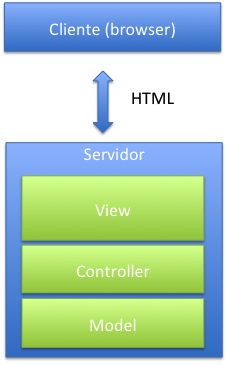
\includegraphics{figuras/server_side_mvc}}
    \caption{Modelo MVC básico}
    \label{submeter}
\end{figure}

Foi se criado um formato um pouco mais rebuscado, mais evoluido e nesse formato tem-se aplicações onde o html é gerado no lado do servidor, mas foi criada uma técnica conhecida
por muitos como ajax, para atualizar partes de páginas ou até mesmo funcionalidades implementadas para melhorar o desempenho do usuário evitando um reload completos
da página a cada iteração. Contudo ainda neste ponto parte do MVC é executado no lado do servidor e apenas a parte das Views são executadas no lado do cliente. Este modo eram
chamado de hibrido por muitos.

\begin{figure}[ht]
    \centering
    \scalebox{0.4}{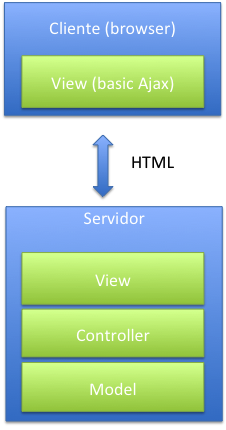
\includegraphics{figuras/hibrid_mode_mvc}}
    \caption{Modelo MVC hibrido}
    \label{submeter}
\end{figure}

Depois de muito se estudar o conceito de modelo MVC - Standard e MVC - hybrid um terceiro modelo surgiu e é nesse que as aplicações client-side executam atualmente e neste a arquitetura
MVC é toda executada em client-side (Lado do clientte ). O Model passa ter entretanto duas atribuições de responsabilidade, a de fornecer toda a API bem como as validações executadas no
lado do servidor, e outra que é executada no lado do cliente que também oferece validações sobre a estrutura do modelo exibido.
\\\\\\
\begin{figure}[ht]
    \centering
    \scalebox{0.4}{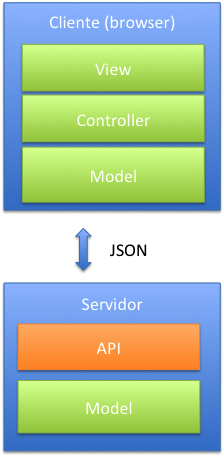
\includegraphics{figuras/client_side_mvc}}
    \caption{Modelo MVC Client-Side}
    \label{submeter}
\end{figure}

Desenvolver aplicações voltadas para client-side possuem algumas vantagens importantes como:
\begin{itemize}
    \item{ \textbf{Melhor desempenho para o usuário:}
      sendo esta uma das principais vantagens no que diz respeito ao desempenho de cada browser, não ter que precisar 
      fazer requisições a todo momento, na hora de fazer dowload, ou atualizar a página completa a cada iteração do 
      usuario com esta. Aplicações feitas em client-side funcionam tao bem quanto aplicações feitas para desktop.
    }
    \item{ \textbf{Melhor desempenho na transferência de dados:}
      Há também um ganho considerável na taxa de transmissão dos dados, ao invés de carregar o cenário da página html completa
      a cada interação do usuário, na arquitetura client-side todo o cenário é transferido na primeira solitação e as requisições 
      seguintes são responsáveis por trafegar apenas os dados consolidados entre o cliente e o servidor, normalmente no formato JSON. 
    }
    
    \item{ \textbf{Facilidade de manutenção:}
      com aplicações em client-side a API forncecida pelo servidor possibilita a facilidade de manutenção de forma independente ao usuário,
      de tal forma que o cliente não perceberá quando a página sofrer atualizações em tempo não real.
    }
    
    \item{ \textbf{Redução de carga no lado do Servidor:}
      O sistema completo passa a ser enviado ao usuário final através de arquivos html, css e javascript que podem ser comprimidos 
      e distribuídos através de CDN's com faclidade. Uma vez baixados esses arquivos são mantidos em cache no browser da preferência do usuário. 
      O servidor tem a responsabilidade apenas de fornecer uma API, enviar e receber os dados no formato JSON. Dessa forma todo o processamento 
      é responsável por particionar dos dados e  a geração de templates fica exclusivamente no lado cliente e não mais no servidor, liberando recursos. 
    }
\end{itemize}

\section{Ruby On rails}

RoR é um web framework escrito sob a linguagem Ruby. Criado por \cite{DAVIDHANSSON} em 2003, baseado em seu trabalho no Basecamp, que é 
uma ferramenta de gerenciamento de projetos 37 signals. No entanto David só lançou o RoR como código aberto em julho de 2004, e mais tarde em dezembro de 
2005 foi lançada a primeira versão do Ruby on Rails.

Assim como outros frameworks de aplicação web o RoR utiliza a arquitetura  MVC(model view controller), fornecendo um isolamento entre a lógica de negócio 
dos modelos, a interface com o usuário através das views e a manipulação de todas as requisições no servidor de apicação. O que contribui muito para que a manutenção do código seja bem mais fácil e flexível.

Ruby on Rails possui uma filosofia que segue dois princípios:
\begin{itemize}
 \item {DRY}
 \item {CoC}
\end{itemize}

\subsection{DRY}
Don't Repeat Yourself(Não se repita). Se aplicado corretamente, possibilita a reduzir a duplicação de tarefas dentro de um projeto. Réplicas ou duplicatas de qualquer
tipo, dentro de uma aplicação, leva a dificuldade de modificação e manutenção e inconsistência, sem levar em conta em alguns casos a ilegibilidade do source-code. 
Em RoR, se pode ver este princípio em ação em quase tudo, desde as componentes reutilizáveis em forma de plug-ins para a forma como as tabelas da base de dados escolhida são mapeadas.

\subsection{CoC}

\textit{Convenção sobre Configuração} ou \textit{programação por convenção} vem do termo em inglês \textbf{(Convention over Configuration - CoC)}, uma prática de desenvolvimento de software que visa diminuir o nnumero obsoleto de decisões que os desenvolvedores precisam tomar ao longo de seus projetos. Estabelecendo simplicidade sem preder flexibilidade.
Quando um desenvolvedor seja ele experiente ou não for iniciar atividades em Rails, o usuário estará sempre na maior parte do tempo interagindo com os controllers, views e models entre outras palavras a arquitetura MVC amplamente vista em design patterns e além desse fator importante estara diretamente conectato para a base de dados escolhida seja ela 
relacional ou não relacional como no caso dos NoSQL. De tal forma a reduzir a necessidade de configuração pesada.

RoR permite a criação de regras personlizadas, contudo é sempre  uma boa idéia usar as convenções que o própio	Rails oferece, essas convenções deverão acelerar o desenvolvimento, manter um código limpo, conciso e legível e o mais importante estas convenções permitem uma navegação muito mais fácil dentro da aplicação.
Rails não foi baseado  em um único padrão de desenvolvimento, mas sim uma série de padrões. Outros frameworks que faziam parte do núcleo do Rails antigamente foram removidos desse núcleo afim de reduzir o acoplamento e com isso e permitir que quem o esteja utilizando os substituam sem  muita dificuldade, mas continuam funcionando e sendo usados em conjunto. Aqui estão alguns deles:

\subsection{Active Record}
Para se entender este item sendo este um dos mais importantes para se construir uma aplicação em Rails é necessário compreender um dos fundamentos mais criteriosos em orientação a objetos
o conceito de ORM(Object-Ralational Mapping) que pode ser traduzido como Mapeamento Objeto Relacional e segundo \cite{TECTARGET}, trata-se de uma forma rapida e prática de relacionar e endereçar, e manipular objetos sem que seja, necessário se preocupar com a forma ao qual estes se comunicam e se relacionam entre si.
ORM possibilita aos desenvolvedores experientes ou novatos à manter a uma perspectiva consistente dos objetos no percurso do projeto, mesmo que haja alteraçãoes no código ou até mesmo na base de dados em questão.

De acordo com \cite{BAKHARIA}, o \textbf{Active Record} cria uma abstração de \textit{OODB} - \\ (Orientação a Objeto em Banco de dados) onde o rails cria um mapeamento relacional entre tabelas e classes do modelo ao qual estas pertencem. Sendo que o Active Record também fornece uma série de métodos nas próprias classes para trabalhar com a manipulação de dados, como por exemplo criar, salvar, atualizar, deletar, entre outras palavras todas operações para gerenciar o CRUD do modelo descrito.
Ao contrário de outras bibliotecas complexas o Active Record não necessita de configurações desse nível, além de ser capaz de se dispor da capacidade de propor mapeamentos objeto relacional com base em convenções de nomenclatura de tabelas e nome dos campos o que ajuda a justificar a importância do conceito chave de desenvolvimento a idéia de \textit{ Convention Over Configuration(Convenção Preferível à Configuração) } o que a mesma afirma que com esse pretexto o Active record torna o Ruby On Rails uma das ferramentas de desenvolvimento web mais ágil para a produção de sistemas com banco de dados.

Na Prática todo e qualquer modelo criado pelo gerador de componentes do rails o mesmo estende a classe nativa \textbf{ActiveRecord::Base} responsável por abstrair uma entidade contida na base de dados, assim como cada objeto representa uma linha do banco de dados como menciona \cite{PRAGMATICRUBY}.

\subsection{Action Controller}
Segundo \cite{ORSINI}, em qualquer aplicação feita em rails, um controller é uma especialização da classe \textbf{Action Controller} que oferece uma série de conjunto de regras de negócio para a aplicação
Geralmente cada controller responde ao modelo ao qual encontra-se alocado, podendo este ser o que muitos chamam de \textbf{Controller Virtual}. Um Controller Virtual também é chamado de controller genérico, 
que não necessáriamente está associado à um modelo.

\subsection{Action View}
Segundo \cite{BAKHARIA}, Action View é um dos componentes responsável apenas por gerar a interação entre a aplicação e o usuário. Um Controller pode ter várias actions( métodos ), e para cada action dependendo da situação uma view para esta que automáticamente é reconhecida e exibida.
Um action view também é conhecida como template. Esse template pode reproduzir vários elementos, não só o html, mas também outros tipos como XML, JavaScript, PDF.
O template nada mais é do que uma renderização de código ruby com Html e possivelmente Javascript.


\subsection{Action Support}
"Active Support é composto por uma série de bibliotecas compartilhadas por todos os componentes gerenciados pelo Rails. 
Muito do que está acoplado nesse módulo está destinado a uso interno do Rails.
No entanto, Active Support também estende algumas das classes internas de Ruby de maneira útil e interessante."\cite{PRAGMATICRUBY}.

\subsection{Action Mailer}
ActionMailer é um componente nativo do rails que permite que a aplicação desenvolvida possa enviar correio-eletrônico. 
\\
"É importante um sistema que facilite a operação de envio de mensagens de e-mails porque
essa é uma operaão tem diversas aplicações comuns como: Enviar e -mails de confirmação de
cadastro; Notificações de erros ao administrador do site; Confirmação de compra de produtos
em lojas virtuais; Newsletters".\cite{BAKHARIA}
\\
\noindent A classe Mailer do Rails possui métodos para diferentes formas de enviar mensagens de acordo com o que a aplicação necessita. O formato de saida dessa mensagem
e descrito em sua ActionView de forma muito similar com as actions views gerenciadas pelos erb.

\subsection{Scaffolding}
Rails possui uma ferramenta de desenvolvimento ágil conhecida como scaffold, e essa ferramenta possibilita a criação do Model de acordo com os parâmetros expecificados.
Este comando possibilita a criação de todo o CRUD, controller, model e views deste modelo dito no ato da criação. Em uma aplicação rails dependende do que se deseja e dependendo 
da não complexidade o scaffold se faz uma boa escolha e para utiliza-lo basta usar:

{\singlespace
\begin{lstlisting}[caption=Exemplo de uso de scaffold, language=Ruby,label={scaffold}]
  >> rails g scaffold user username:string address:string birth_date:date
\end{lstlisting}
}

Em uma aplicação rails é sempre bom fazer uso de CoC, e nessas convenções o rails tem uma nomenclatura no que diz respeito a \textbf{controllers e models}, toda vez que um controller é criado
este sempre estará no plurar, já o model correspondente irá sempre estar no singular. Isto quando for utilizado o comando scaffold que no ato irá gerar uma série de outros arquivos além do controller, 
do model e das views responsáveis por gerenciar o modelo descrito. 
\begin{figure}[ht]
    \centering
    \scalebox{0.4}{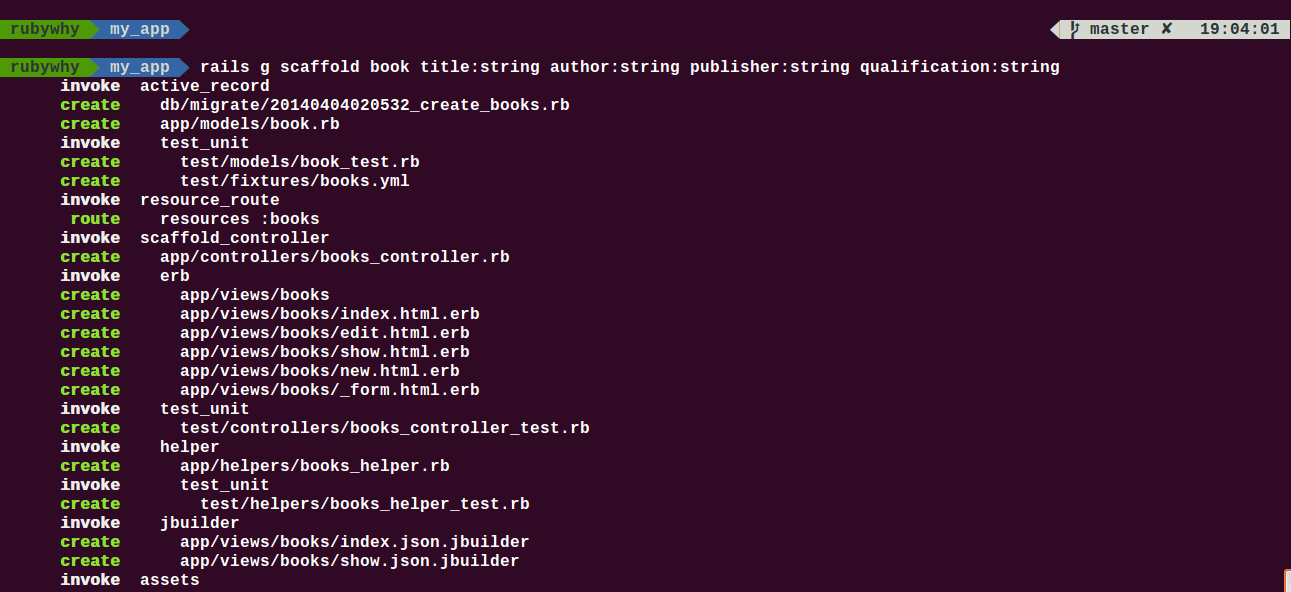
\includegraphics{figuras/scaffold_generator}}
    \caption{Parte dos arquivos criados após o scaffold.}
    \label{submeter}
\end{figure}
\\

A introdução deste comando \textit{rails g} possibilita ao desenvolvedor uma série de outros comandos
uma vez que pode ser abreviado, o nome por extenso para este comando é \textbf{generate}. O generate é o gerador de elementos do rails, com ele é possivel realizar outras 

\subsection{Migrations}
O Migration pertime alterar o esquema de banco de dados ao longo do tempo de uma forma consistente e fácil.
Ele utiliza uma DSL do ruby para que nao tenha que escrever SQL a mão, fazendo assim com que as mudanças no banco de dados
seja independente. Cada migration é uma nova "versão" do banco de dados. Um esquema começa vazio e a cada migration ele é modificado
para acrescentar ou remover tabelas, colunas ou entradas necessárias.

\subsection{Rake}
Rake é conhecido como Ruby Make, um utilitário autônomo Ruby que substitui o utilitário Unix 'make'
e usa um "Rakefile' e arquivos com extensão .rake para criar uma lista de tarefas. No Rails, Rake é
usado para tarefas comuns de administração, especialmente os mais sofisticados que constroem fora de si.
Pode-se obter uma lista de tarefas Rake disponíveis simplesmente digitando rake - tasks.
Cada tarefa tem uma descrição, o que deve ajudar a encontrar funções expecificas para o que se deseja

\subsection{Organização de arquivos em Rails}
RoR se dispõe de ferramentas de desenvolvimento rápido e sem muito esforço. Para se iniciar uma nova aplicação em rails
bastaria usar o comando inicial:

{\singlespace
\begin{lstlisting}[caption=Exemplo de uso de scaffold, language=Ruby,label={scaffold}]
  >> rails new my_new_rails_app [ -d  ] { options }
\end{lstlisting}
}

Ao utilizar esse comando inicial toda uma estrutura de arquivos e diretórios é criada. 

\begin{figure}[ht]
    \centering
    \scalebox{0.4}{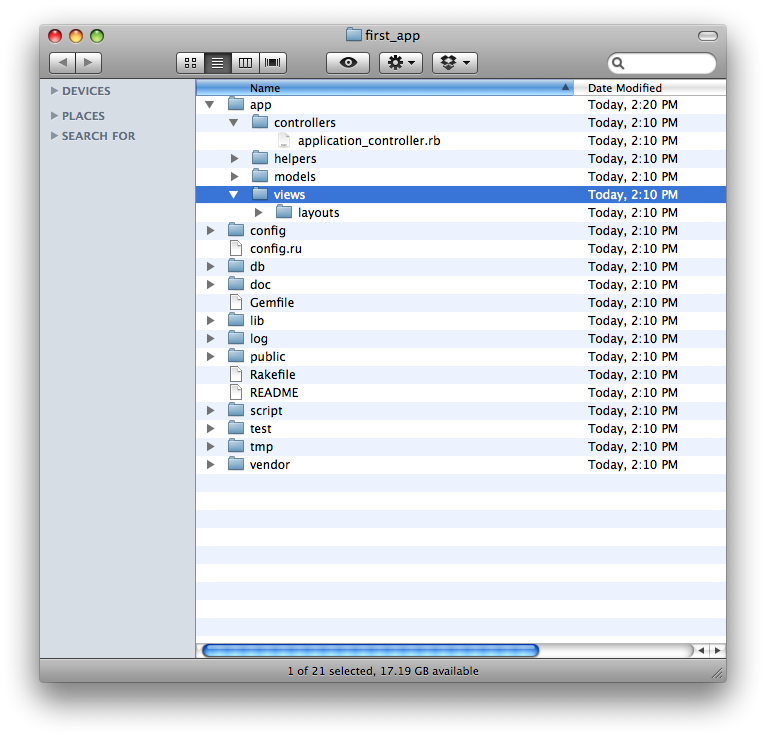
\includegraphics{figuras/rails_app}}
    \caption{Estrutura básica de arquivos e diretórios}
    \label{submeter}
\end{figure}

É possivél ainda passar parametros para a criação da mesma tais como:
o -d siguinifica qual a base de dados a ser utilizada, RoR possui três ambientes de integração: \textbf{development} responsável apenas pela etapa de desenvolvimento, 
este recarrega todas as classes sempre que uma nova action é requisitada, portanto uma nová cópia da classe é obtida, incluido qualquer alteração recente na mesma,
\textbf{test} - o próprio nome similar ao nosso português já indica que este é um ambiente onde se pode criar os testes contidos na aplicação que see tornarão a documentação
executavel da aplicação desenvolvida e por ultimo RoR possui um ambiente - \textbf{production} - onde o RoR carrega a classe apenas uma única vez, é onde a aplicação irá rodar em produção constante em um servidor de aplicação,
sem a necessidade de sofrer alterações como normalmente é feito em desenvolvimento. Ainda existe uma série de parametros que se pode passar para a criação de uma aplicação em rails uma delas é a opção de usar ou não o ActiveRecord
que é nativo do rails ao utilizar "\textbf{--skip-active-record}" o desenvolvedor está explicitamente dizendo ao rails para criar uma aplicação sem persistência à uma base de dados relacional, com isso é possivel escolher alguma das
base de dados NoSQL como por exemplo MongoDB, CouchDB, Cassandra etc.

\section{Git}
Git é um sistema de controle de versões distribuídas livre e de código aberto, projetado para lidar com qualquer projeto, desde o menor ao maior com rapidez e eficiência \cite{SOFTWARE-FREEDOM-CONSERVANCY}.

A historia do Git está muito relacionada a criação do Linux e de Linus Torvalds, seu criador, bem como com toda comunidade de desenvolvimento Linux. Durante anos a comunidade utilizou a ferramenta \textit{BitKeeper} para guardar a modificações do projeto.

Em 2005, após um problema com a proprietária deste, a comunidade decidiu criar sua própria ferramenta a partir da experiência com a anterior, houve um novo foco em: velocidade, \textit{design} simples, suporte para desenvolvimento paralelo, distribuição completa e a habilidade necessária para lidar com projetos grandes sem perda de velocidade e dados.

Assim, esse novo sistema de versionamento permite que qualquer repositório seja o centro do versionamento, deixando todo \textit{log} das modificações guardados nele sem que para isso precise de uma conexão a rede ou servidor geral.
\chapter{CLOUDOOO}
\thispagestyle{empty}

Em função da necessidade da conversão de documentos a empresa francesa Nexedi SA originou a construção da ferramenta OpenOffice.Org Daemon (OOOD), entretanto seu uso prolongado apresentou erros que precisavam de tratamento e ainda com novas demandas crescendo era necessário a realização de mudanças e até de uma nova ferramenta mais estável. Em parceria com o NSI, foi idealizado o desenvolvimento desta nova ferramenta.

O resultado da continuação do desenvolvimento foi a ferramenta OOOD 2.0, posteriormente nomeada por CloudOoo, apresentada em 2010. Esta nova versão da ferramenta se provou bem mais estável no uso a longo prazo, embora fosse considerada mais lenta em processos individuais, devido aos tratamentos adicionados para os erros conhecidos, e suas modificações de novas funcionalidades.

Ao final do processo de melhoria da ferramenta, novas funcionalidades foram idealizadas para diferentes tipos de arquivos, tais como arquivos de áudio, vídeo, imagem e PDF. A princípio essas funcionalidades seriam as mesmas aplicadas a documentos, conversões e manipulações gerais, vindo a criação de funcionalidades especificas quando a ferramenta fosse considerada estável.

Assim o CloudOoo apresentado neste capítulo, é um serviço Web livre e de código aberto, sob a licença LGPL, que foi desenvolvido através parceria da Nexedi e do NSI, na linguagem de programação Python e que utiliza o protocolo XML-RPC para troca de mensagens, que pode ser utilizado inteiramente ou em partes separadas.

\section{Estrutura}

Desde de sua estrutura anterior, o CloudOoo foi desenvolvido para trabalhar de forma genérica prevendo futuras mudanças. Sua estrutura contém as interfaces:

\begin{itemize}
    \item{IApplication: representa os métodos de controles as aplicações externas do servidor;}
    \item{IFile: representa métodos para manipulação dos arquivos recebidos;}
    \item{IOdfDocument: representa métodos de manipulação específica de documentos ODF;}
    \item{IHandler: representa os objetos que irão realizar a requisição emitida pelo cliente;}
    \item{IMonitor: representa métodos de controle e manuseio dos processos estabelecidos no servidor;}
    \item{IMimemapper: representa métodos utilizados para trabalhar com filtros;}
    \item{IFilter: representa métodos de tratamento de filtros;}
    \item{ILockable: representa os métodos de controles para região crítica do servidor;}
    \item{ITableGranulator: representa métodos para extrair tabelas de documentos;}
    \item{IImageGranulator: representa métodos para extrair imagens de documentos;}
    \item{ITextGranulator: representa os métodos para extrair o conteúdo de um documento em capítulos e parágrafos;}
    \item{IERP5Compability: representa os métodos de compatibilidade com o ERP5;}
    \item{IManager: representa os métodos utilizáveis entre cliente e servidor.}
\end{itemize}

As próximas subseções apresentam detalhadamente sobre cada interface e as principais classes a implementá-las.


\subsection{ILockable}
\label{ilock}

Quando se possui-se um recurso compartilhado, isto é, um recurso representado por outra aplicação rodando em paralelo à aplicação principal, admiti-se também existir uma região crítica.

Esta visão ocorre devido ao fato que determinadas aplicações não conseguem atender a mais de um processo simultaneamente, assim é necessário controlar essa região crítica prevendo travá-la caso um processo já esteja em usando a mesma.

Com este intuito a interface ILockable foi implementada.


\subsection{IApplication}
\label{iapplication}

Por possuir a opção instalação em um ambiente dedicado onde tanto o CloudOoo, quanto suas ferramentas podem possuir instalação própria, a partir do uso do Buildout, foi preciso construir uma interface para controlar as funções dos processos utilizados pela aplicação, ou seja, uma classe que fosse capaz de carregar a configurações das aplicações, controlar a inicialização e finalização de cada processo, e que fosse capaz de verificar se continuavam rodando no sistema operacional, a partir de um identificador e/ou da porta que cada uma utilizasse.


\subsubsection{Application}
\label{application}

Esta classe implementa a interface IApplication e tem por objetivo controlar processos externos que estejam sendo utilizados dentro do CloudOoo, como o por exemplo os processos do LibreOffice que precisam estar iniciados para possibilitar a manipulação dos documentos.

Além dos métodos citados em \ref{iapplication} esta classe é capaz de apresentar erros ocorridos durante processos e também de retornar o \textit{pid} utilizado pela aplicação. E ainda um método responsável pelo endereço dessa aplicação, ou seja, onde esta estabelecida e em qual porta.

No código \ref{application} existe uma parte da implementação desta classe, em que é exibido como retornar o \textit{pid} de cada processo. No código é possível notar o uso da biblioteca \textit{implements} do Zope.Interface, utilizada para implementar a interface IApplication.

{\singlespace
\begin{lstlisting}[caption=Trecho de código referente a função de pid,language=python,label={application}]
from zope.interface import implements
from cloudooo.interfaces.application import IApplication

class Application(object):

  implements(IApplication)

  name = "application"

  def pid(self):
    if not hasattr(self, 'process'):
      return None
    return self.process.pid
\end{lstlisting}
}

\subsubsection{OpenOffice}
\label{ooffice}


A classe OpenOffice foi exclusivamente criada visando controlar a aplicação LibreOffice, anteriormente conhecida por OpenOffice.Org, a qual foi responsável por maior parte dos erros obtidos no CloudOoo. 

Esta classe estende o uso da interface IApplication, seção \ref{application} e ainda implementa a interface ILockable, \ref{ilock}, para que assim seja possível controlar a aplicação, trancá-la e destrancá-la durante seu processo de uso.

A partir do método \textit{isLocked}, \ref{lockoffice}, é possível verificar se esta aplicação está trancada ou disponível para uso, evitando assim erros, como o \textit{deadlock} por exemplo. Este método realiza uma consulta por meio da função \textit{locked} implementada pela classe Lock, nativa do Python, e própria para trabalhar com Threads.

{\singlespace
\begin{lstlisting}[caption=Trecho isLocked da classe OpenOffice,language=python,label={lockoffice}]
from threading import Lock

class OpenOffice(Application):

  implements(ILockable)

  def __init__(self):
    self._bin_soffice = 'soffice.bin'
    self._lock = Lock()
    self._cleanRequest()

  def isLocked(self):
    return self._lock.locked()
\end{lstlisting}
}


\subsection{IFile}
\label{ifile}

Esta interface propõe um contrato de tratamento de arquivos, a fim de assegurar uma resposta eficiente e consistente ao cliente. Nela são contidos métodos para que o conteúdo do arquivo seja guardado durante sua instânciação de forma no acontecimento de erros não previstos este conteúdo pode ser recuperado, ou mesmo restaurado a forma original.


\subsubsection{File}
\label{file}

Com base na implementação da interface IFile, esta classe possui métodos para manter qualquer arquivo recebido do cliente no sistema apenas durante o uso do mesmo.

Ao receber um arquivo ela escreve o mesmo no disco, podendo assim recuperar seus dados, e obter informações do mesmo, como seu caminho, por exemplo. No código \ref{file} existe uma representação de como cada File é recriado.

{\singlespace
\begin{lstlisting}[caption=Trecho de criação da classe File,language=python,label={file}]
import tempfile
from zope.interface import implements
from cloudooo.interfaces.file import IFile

class File(object):

  implements(IFile)

  def __init__(self, base_folder_url, data, source_format):
    self.base_folder_url = base_folder_url
    self.directory_name = self._createDirectory()
    self.original_data = data
    self.source_format = source_format
    self.url = self.load()

  def _createDirectory(self):
     return tempfile.mkdtemp(dir=self.base_folder_url)
\end{lstlisting}
}

Para identificar o diretório do File, é utilizado o \underline{base folder url} o qual se refere a pasta base informada pelo próprio usuário em questão, além do \textit{mkdtemp} que cria um diretório temporário para esta nova instância. 

Após o uso deste arquivo, o File é instituído a remover a instância do sistema, bem como qualquer arquivo criado a partir desta a fim de não esgotar o servidor com arquivos desnecessários.


\subsection{IOdfDocument}

Embora muito similar a interface IFile, seção \ref{ifile}, porém seu tratamento é especifico para documentos ODF, dada a complexidade de armazenamento e manipulação destes.

\subsubsection{Document}

Por ter sido inicialmente desenvolvido para documentos ODF a estrutura do CloudOoo é relativamente planejada para estes, que por possuírem uma estrutura complexa e compacta exigiram a criação de classes especificas. 

Como no caso do Document, o qual tem seus métodos desenhados com base em estudos anteriores sobre estruturas XML e sobre a manipulação de documentos ODF.

Assim, no código \ref{document}, esta um trecho do código desta classe que visa a estruturação de um documento ODF com base no uso do ZipFile para ordernar seu XML através da obtenção do conteúdo de ``content.xml''.

{\singlespace
\begin{lstlisting}[caption=Trecho de estruturação do content.xml,language=python,label={document}]
from zope.interface import implements
from zipfile import ZipFile
from StringIO import StringIO
from lxml import etree
from cloudooo.interfaces.file import IOdfDocument


class OdfDocument(object):

  implements(IOdfDocument)

  def __init__(self, data, source_format):
    self._zipfile = ZipFile(StringIO(data))
    self.source_format = source_format
    self.parsed_content = etree.fromstring(self.getContentXml())

  def getContentXml(self):
    return self._zipfile.read('content.xml')
\end{lstlisting}
}


\subsection{IMonitor}

Esta interface foi desenvolvida principalmente com base nos erros anteriormente obtidos com o uso do LibreOffice, no entanto é importante para o sistema como um todo.

Seu uso estabelece controles sobre princípios básicos do sistema, como uso de memória, tempo de requisições, tempo de uso do processo, entre outros.


\subsubsection{Monitor}
\label{mon}

Basicamente a classe Monitor funciona como uma simples implementação da interface IMonitor a fim de estabelecer seus atributos principais, como por exemplo o tempo mínimo entre a monitorações do sistema(\textit{interval}), que se pode notar no código \ref{monitor}. 

Além deste, outro atributo essencial é a instância de OpenOffice, \ref{ooffice}, através da variável \textit{openoffice}.

{\singlespace
\begin{lstlisting}[caption=Inicialização da classe Monitor,language=python,label={monitor}]
zope.interface import implements
from cloudooo.interfaces.monitor import IMonitor

class Monitor(object):

  implements(IMonitor)

  def __init__(self, openoffice, interval):
    self.status_flag = False
    self.openoffice = openoffice
    self.interval = interval

\end{lstlisting}
}

As próximas subseções explicam detalhadamente sobre estes controles através da herança desta classe.

\subsubsection{MonitorMemory}
\label{monitormem}

Nas configurações do CloudOoo existem definições que podem ser modificadas de acordo com o sistema em que vai ser instalado, entre elas existe uma variável responsável pelo uso máximo de memória pelo LibreOffice.

A partir dessa definição, dada em \textit{megabytes}, a MonitorMemory monitora o uso da memória do sistema pela variável \textit{limit}, vista em \ref{mmem}. Assim caso este limite máximo seja atingido, a aplicação é reinicia com intuito de limpar da memória mensagens trocadas e que não foram liberadas de uso da mesma, evitando assim o evento chamado \textit{memory leak}, o qual consiste no uso de toda memória do sistema.

{\singlespace
\begin{lstlisting}[caption=Trecho de criação da classe MonitorMemory,language=python,label={mmem}]
from monitor import Monitor
from multiprocessing import Process
from time import sleep

class MonitorMemory(Monitor, Process):

  def __init__(self, openoffice, interval, limit_memory_usage):
    Monitor.__init__(self, openoffice, interval)
    Process.__init__(self)
    self.limit = limit_memory_usage
\end{lstlisting}
}

Além de Monitor, \ref{mon}, estas subclasses também implementam a classe Process, nativa do Python, que tem por função ser o controle dos processos iniciados no sistema pela aplicação;

\subsubsection{MonitorTimeout}
\label{monitortim}

Através da definição citada na subseção \ref{monitormem}, o MonitorTimeout realiza uma comparação de tempo ativo da aplicação em função do \textit{interval} para estabelecer o chamado \textit{timeout}, isto é, o tempo limite de execução de um determinado processo.

Caso este tempo seja excedido a aplicação é forçada a parar, sendo reiniciada posteriormente, \ref{mtim}.A utilidade desta limitação é dada pela idéia de que caso este tempo tenha excedido ocorreu algum erro durante o processo, provavelmente em função da resposta da aplicação, assim reiniciá-la pode resolvê-lo.

{\singlespace
\begin{lstlisting}[caption=Método run da classe MonitorTimeout,language=python,label={mtim}]
from monitor import Monitor
from multiprocessing import Process
from time import sleep

class MonitorTimeout(Monitor, Process):

  def run(self):
    sleep(self.interval)
    if self.openoffice.isLocked():
      self.openoffice.stop()
\end{lstlisting}
}

A utilidade desta limitação é dada pela idéia de que caso este tempo tenha excedido ocorreu algum erro durante o processo, provavelmente em função da resposta da aplicação, neste caso o OpenOffice. Assim reiniciá-la pode resolver tal erro.


\subsubsection{MonitorSleepingTime}

Com intuito de poupar uso do sistema em momentos desnecessários esta classe foi criada para observar o momentos de inutilização da aplicação e para parar a mesma nestes momentos.

A partir de uma definição inicial para o tempo de inutilização, definida na instalação do CloudOoo (\underline{sleeping time}), o MonitorSleepingTime ``trancar'' a aplicação, linha 11, e para sua execução para enfim destrancá-lo caso algum processo queira utilizar a aplicação, \ref{mstime}.

Assim é possível economizar no uso de recursos, e disponibilizá-los para outras aplicações que possam vir a utilizar o mesmo.

{\singlespace
\begin{lstlisting}[caption=Método run da classe MonitorSleepingTime,language=python,label={mstime}]
from monitor import Monitor
from threading import Thread
from time import sleep, time

class MonitorSleepingTime(Monitor, Thread):

  def run(self):
    while self.status_flag:
      current_time = time()
      if self.openoffice.status() and\
        (self._touched_at + self.sleeping_time) <= current_time:
        self.openoffice.acquire()
        self.openoffice.stop()
        self.openoffice.release()
      sleep(self.interval)
\end{lstlisting}
}

\subsubsection{MonitorRequest}

A fim de conservar a estabilidade do CloudOoo, o MonitorRequest implementa um controle em função do valor máximo de requisições (\underline{request limit}), isto é, um número máximo de requisições do cliente que podem ser respondidas por cada instância da aplicação no servidor.

Caso o valor informado seja excedido a instância é encerrada, em seguido uma nova instância da mesma aplicação é iniciada, como visto em \ref{mreq}.

{\singlespace
\begin{lstlisting}[caption=Método run da classe MonitorRequest,language=python,label={mreq}]
from monitor import Monitor
from threading import Thread
from time import sleep


class MonitorRequest(Monitor, Thread):

  def run(self):
    while self.status_flag:
      if self.openoffice.request > self.request_limit:
        self.openoffice.acquire()
          self.openoffice.getAddress())
        self.openoffice.restart()
        self.openoffice.release()
      sleep(self.interval)
\end{lstlisting}
}

\subsection{IMimemaper}

Em casos de aplicações como o LibreOffice que representam uma suíte de menores utilitários é preciso reconhecer a extensão de arquivo específica para cada utilitário. 

De forma geral estas extensões são explicitas no nome do arquivo. Entretanto, caso de que esta não sejam explicitas, é preciso reconhecer o tipo de arquivo de alguma outra forma. 

Neste caso existem o \textit{mimetypes}, que são identificadores presentes no conteúdo do arquivo, que permitem decidir sua extensão. 

Esta interface propõe métodos ara lidar com a identificação desses \textit{mimetypes}.

Seu exemplo de uso é a classe Mimemapper a qual será apresentada na próxima subseção.


\subsubsection{Mimemapper}
\label{mimemapper}

O CloudOoo possui seus próprio filtros para identificar e renderizar arquivos dentro de sua própria instância.

No entanto, dada a necessidade de suas aplicações internas, tornou-se necessário identificá-los de forma a torná-los igualmente reconhecível dentro de cada aplicação específica.

No caso do LibreOffice é possível, através do uso do UNO, extrair os \textit{mimetypes} e demais informações como filtros próprios para  esta aplicação. Um vez extraídos é importante definí-los numa inicialização, \ref{mmapper}.

{\singlespace
\begin{lstlisting}[caption=Trecho de criação da classe Mimemapper,language=python,label={mmapper}]
from zope.interface import implements
from cloudooo.interfaces.mimemapper import IMimemapper

class MimeMapper(object):

  implements(IMimemapper)

  def __init__(self):
    self._loaded = False
    self._filter_by_extension_dict = {}
    self._extension_list_by_type = {}
    self._doc_type_list_by_extension = {}
    self._mimetype_by_filter_type = {}
    self._document_type_dict = {}
\end{lstlisting}
}

Assim uma vez que tenham sido definidos os filtros não é necessário saber a extensão do arquivo por extenso.


\subsection{IFilter}

Citados na seção anterior, \ref{mimemapper}, os filtros podem ter demais propriedades que ao serem requisitadas precisam estar disponível de forma facilmente utilizável.

Com base neste principio de utilização, esta interface propõe um contrato para trabalhar com os filtros mais complexos da melhor forma possível e igualmente da forma mais simples.


\subsubsection{Filter}

Se comparada as outras classes e suas devidas interfaces, a classe Filter pode ser considerada a que representa um dos métodos mais simples.

Ao ser iniciada ela guarda todos os dados de cada filtro em diversos atributos que foram selecionados prevendo seu uso posterior na aplicação, \ref{filt}.

{\singlespace
\begin{lstlisting}[caption=Trecho de criação da classe File e método getDocumentService,language=python,label={filt}]
from zope.interface import implements
from cloudooo.interfaces.filter import IFilter

class Filter(object):

  implements(IFilter)

  def __init__(self, extension, filter, mimetype, document_service, **kwargs):
    self._extension = extension
    self._filter = filter
    self._mimetype = mimetype
    self._document_service = document_service
    self._preferred = kwargs.get('preferred')
    self._sort_index = kwargs.get('sort_index')
    self._label = kwargs.get("label")

  def getName(self):
    return self._filter

  def getDocumentService(self):
    return self._document_service
\end{lstlisting}
}

Apesar de simples essa classe possui métodos de extrema importância, como \textit{getDocumentService}, linha 10 \ref{filt}, que no caso do LibreOffice retornar qual aplicação será utilizado para aquela instância.

\subsection{IHandler}
\label{ihandler}

Esta interface foi especificamente criada para estabelecer o contrato entre as aplicações externas utilizadas pelo servidor em função dos pedidos do cliente no que desrespeito a manipulação direta do arquivo, como no caso de conversões por exemplo, ou então extrações e inserções de metadados, respectivamente os métodos de \textit{convert, getMetadata} e \textit{setMetadata}.

Para as classe que implementam esta interface é recomendado o igual uso de objetos do tipo File, seção \ref{file}, para manipulação dos tipos de arquivos de cada uma dessas.


\subsubsection{OOHandler}

Inicialmente nomeado em função do OpenOffice.Org, este \textit{handler} é uma implementação específica de comunicação com o LibreOffice, que trata de requisições especificas a documentos a fim de manipulá-los.

{\singlespace
\begin{lstlisting}[caption=Trecho de criação da classe OOHandler,language=python,label={oohand}]
from cloudooo.interfaces.handler import IHandler
from cloudooo.handler.ooo.mimemapper import mimemapper
from cloudooo.file import File
from cloudooo.handler.ooo.monitor.timeout import MonitorTimeout
from cloudooo.handler.ooo.monitor import monitor_sleeping_time
from psutil import pid_exists


class Handler(object):

  implements(IHandler)

  def __init__(self, base_folder_url, data, source_format, **kw):
    self.document = File(base_folder_url, data, source_format)
    self.zip = kw.get('zip', False)
    self.uno_path = kw.get("uno_path", None)
    self.office_binary_path = kw.get("office_binary_path", None)
    self.timeout = kw.get("timeout", 600)
    self.refresh = kw.get('refresh', False)
    self.source_format = source_format
    if not self.uno_path:
      self.uno_path = environ.get("uno_path")
    if not self.office_binary_path:
      self.office_binary_path = environ.get("office_binary_path")
\end{lstlisting}
}

No código \ref{oohand} é possível notar a incorporação de outras classes como File \ref{file}, utilizada para salvar o arquivo recebido em sistema; MimeMapper \ref{mimemapper} para controlar os filtros do LibreOffice; e MonitorTimeout \ref{monitortim} para controlar o tempo gasto pela aplicação para realizar suas funcionalidades.

\subsubsection{PDFHandler}

Por utilizar de duas ferramentas, o Poppler e PDFTk, esta classe foi nomeada em função do tipo de arquivo que é responsável, ou seja, arquivos PDF.

{\singlespace
\begin{lstlisting}[caption=Trecho de criação da classe PDFHandler,language=python,label={pdfhand}]
from zope.interface import implements
from cloudooo.interfaces.handler import IHandler
from cloudooo.file import File

class Handler(object):

  implements(IHandler)

  def __init__(self, base_folder_url, data, source_format, **kw):
    self.base_folder_url = base_folder_url
    self.document = File(base_folder_url, data, source_format)
    self.environment = kw.get("env", {})
\end{lstlisting}
}

No código \ref{pdfhand} é possível notar que a implementação desta classe é bem mais simples que a OOHandler \ref{oohand}, por exemplo.
Nela são especificados apenas o diretório (\underline{base folder url}), os dados do arquivo (\textit{document}) e o PATH deste sistema (\textit{environment}), que apontará para os binários do Poppler e PDFTk.


\subsubsection{IMAGEMAGICKHandler}

No que se trata de ferramentas para imagens o ImageMagick é uma das melhores disponível a nível de comando, ela consegue inclusive manipular dados do tipo \textit{Exif}, que são metadados referentes a imagens.

Assim com base na ferramenta que utiliza, esta classe é responsável pela conversão e extração de metadados de arquivos de imagem, visto em \ref{imhand}. Deseja-se ainda implementar uma funcionalidade de inserção destes, no entanto esta funcionalidade requer uma base de estudos maior.

{\singlespace
\begin{lstlisting}[caption=Método getMetadata da classe IMAGEMAGICKHandler,language=python,label={imhand}]
from zope.interface import implements
from cloudooo.interfaces.handler import IHandler

class Handler(object):

  def getMetadata(self, base_document=False):
    """Returns a dictionary with all metadata of document.
    along with the metadata.
    """
    command = ["identify", "-verbose", self.file.getUrl()]
    stdout, stderr = Popen(command,
                          stdout=PIPE,
                          stderr=PIPE,
                          close_fds=True,
                          env=self.environment).communicate()
    metadata_dict = {}
    for std in stdout.split("\n"):
      std = std.strip()
      if re.search("^[a-zA-Z]", std):
        if std.count(":") > 1:
          key, value = re.compile(".*\:\ ").split(std)
        else:
          key, value = std.split(":")
        metadata_dict[key] = value.strip()
    self.file.trash()
    return metadata_dict
\end{lstlisting}
}


\subsubsection{FFMPEGHandler}

O FFMPEG  é capaz de manipular arquivos de áudio e vídeo facilitando assim a criação de uma classe que pudesse ser responsável simultaneamente pela manipulação de ambos.

Assim como as demais classes que implementam o IHandler, esta classe é capaz de manipular os metadados desses arquivos, bem como convertê-los para determinadas extensões do mesmo tipo.

Sendo o FFMPEGHandler uma contribuição direta deste trabalho, é possível encontrá-lo detalhadamente em \ref{ffhand}


\subsection{ITableGranulator, IImageGranulator, ITextGranulator}

Uma das principais funções desenvolvidas para documentos foi a ``granularização'', ela trata da extração de partes importantes de documentos que não sejam especificamente textos, como por exemplo tabelas e imagens. 

Dada a complexidade dessa tarefa foi necessário a implantação das novas interfaces, para que estes processos fossem realizados.

A interface ITableGranulator é a interface responsável pelo processo de ``granularização'' específico de tabelas presentes nos documentos. Ela implementa funções respectivas a uma tabela comum, baseada nas linhas e colunas dessas tabelas.

Na interface IImageGranulator ocorre a ``granularização'' das imagens presentes nestes documentos, que são extraídas em seu formato original, ou em \textit{PNG}.

Por fim através da interface ITextGranulator é possível partir o documento em textos menores dividindo o mesmo a partir de seus parágrafos, ou mesmo em capítulos.

Apesar dessas funcionalidades tratarem diretamente da ``granularização'' de documentos, podemos subdividi-las em dois tipos de documentos: os documentos livres de formato ODF, onde o processo ocorre a partir estudos realizados anteriormente dos mesmos; e documentos PDF, que são igualmente livres, porém tem um tratamento complexo dada sua falta de detalhamento e especificações.


\subsubsection{OOGranulator}

Esta classe foi desenvolvida especialmente para tratar do documentos ODF.

Suas funcionalidades são escritas com base nos \textit{namespaces} encontrados por padrão no XML que compõe esses documentos, no código \ref{namess} é possível ver alguns exemplos desses.

{\singlespace
\begin{lstlisting}[caption=URI e ODF Namespaces,language=python,label={namess}]
TEXT_URI = 'urn:oasis:names:tc:opendocument:xmlns:text:1.0'
TABLE_URI = 'urn:oasis:names:tc:opendocument:xmlns:table:1.0'
DRAWING_URI = 'urn:oasis:names:tc:opendocument:xmlns:drawing:1.0'

TABLE_ATTRIB_NAME = '{%s}name' % TABLE_URI
TEXT_ATTRIB_STYLENAME = '{%s}style-name' % TEXT_URI
DRAWING_ATTRIB_STYLENAME = '{%s}style-name' % DRAWING_URI
DRAWING_ATTRIB_NAME = '{%s}name' % DRAWING_URI
\end{lstlisting}
}

Até o momento essa classe é a única a implementar as exatas três interfaces da subseção anterior.

No trecho abaixo, \ref{gettmatrix}, é possível notar como funciona a pesquisa desta classe por uma tabela especifica a fim de retorná-la ao cliente.

{\singlespace
\begin{lstlisting}[caption=Método de getTableMatrix,language=python,label={gettmatrix}]
  def getTableMatrix(self, id):
    row_list = self.document.parsed_content.xpath(
                        '//table:table[@table:name="%s"]/table:table-row' % id,
                        namespaces=self.document.parsed_content.nsmap)
    if len(row_list) == 0:
      return None

    matrix = []
    for row in row_list:
      matrix_row = []
      for cell in row.iterchildren():
        matrix_row.append(''.join(cell.itertext()))
      matrix.append(matrix_row)
    return matrix
\end{lstlisting}
}


\subsubsection{PDFGranulator}

Esta classe implementa apenas as interfaces ITableGranulator e IImageGranulator, \ref{pdfgran}.

É específica para o tratamento de documentos PDF, que exigem a utilização de bibliotecas e aplicações para ``desmembrá-lo'' e tratar o resultado desta tarefa.

Por não possuir tantas especificações quanto documentos ODF, tratá-lo para ``granularização'' foi uma das contribuições mais complicadas deste trabalho, e no entanto com resultados não tão desejáveis.

\subsection{IManager}

A IManager trabalha como a interface entre o cliente e servidor a fim de estabelecer um protocolo entre ambos.

Ela detém um padrão genérico para troca de informações entre diferentes tipos de arquivos, inclusive vídeos. 

E possui ainda os principais métodos para funcionalidades do CloudOoo, no que desrespeito a todos seus \textit{handlers}, ou seja, módulos para tratar diversos tipos de arquivos.


\subsection{IERP5Compability}

Esta interface estabelece as funcionalidades entre cliente e servidor especificamente para o uso da aplicação ERP5. 

Ela reescreve a chamada dos métodos da aplicação OOOD para utilizarem os novos métodos sem interferir nas requisições feitas pelo uso do ERP5, e outros possíveis clientes que utilizassem a antiga plataforma.


\subsubsection{Manager}
\label{manager}

A classe Manager implementa as classes IManager, IERP5Compability, ITableGranulator, ITextGranulator e IImageGranulator com o propósito de interligar suas funcionalidades ao cliente que venha a requeri-las, em outras palavras esta classe é a principal responsável pela conectividade entre cliente, servidor, aplicação e funcionalidades.

Nela são absorvidos os dados importantes para o funcionamento do CloudOoo, como por exemplo a base de \textit{mimetypes}, os \textit{handlers} disponíveis neste, as pastas de trabalho deste, entre outros dados.

Assim a partir desta classe é possível iniciar o servidor do CloudOoo, \ref{manag}, nela são especificados a pasta de temporários do CloudOoo (\underline{ path tmp dir}), os \textit{mimetypes} registrados (\underline{mimetype registry}), a lista de \textit{handlers} disponíveis nesta instância do CloudOoo (\underline{handler dict}) e por fim a demais variáveis por um dicionário (\textit{kw}).

{\singlespace
\begin{lstlisting}[caption=Inicialização do Manager,language=python,label={manag}]
class Manager(object):
  implements(IManager, IERP5Compatibility, ITableGranulator, IImageGranulator,
             ITextGranulator)

  def __init__(self, path_tmp_dir, **kw):
    self._path_tmp_dir = path_tmp_dir
    self.kw = kw
    self.mimetype_registry = self.kw.pop("mimetype_registry")
    self.handler_dict = self.kw.pop("handler_dict")
\end{lstlisting}
}

\section{Novas Funcionalidades}

Nesta seção encontram-se a funcionalidades diretamente desenvolvidas para o CloudOoo por este trabalho.

Abaixo são listadas todas as contribuições deste trabalho:

\begin{itemize}
    \item{Criação da classe FFMPEGHandler para manipulação de vídeos e áudio;}
    \item{Criação do módulo cloudoooTestCase para testes de serviço;}
    \item{Criação do módulo externo CloudOooTestnode;}
    \item{Criação do módulo externo cloudooo buildout;}
    \item{Manutenção de classes para fins de migração;}
    \item{Criação da classe PDFGranulator;}
    \item{Criação do método granulateFile para granularização de documentos;}
    \item{Manutenção e extensão de código e testes.}
\end{itemize}

As próximas subseções apresentam detalhadamente cada contribuição citada:

\subsection{Criação da classe FFMPEGHandler para manipulação de vídeos e áudio}

Esta foi a primeira funcionalidade desenvolvida por este trabalho e que pode ser explicita desde o ``nível zero".
Assim pretende-se dizer que o CloudOoo não detinha qualquer parte escrita ou planejada para conversão e manipulação de vídeos e áudio antes desta funcionalidade.

\subsubsection{Conversão}

Como o desenvolvimento de todos os \textit{handlers}, a primeira parte deve tratar da conversão direta do tipo de arquivo, que neste caso utiliza a ferramenta FFMPEG:

{\singlespace
\begin{lstlisting}[caption=Conversão do FFMPEGHandler,language=python,label={ffhand}]
from zope.interface import implements
from cloudooo.interfaces.handler import IHandler
from cloudooo.file import File
from subprocess import Popen, PIPE
from tempfile import NamedTemporaryFile

class Handler(object):

  implements(IHandler)

  def __init__(self, base_folder_url, data, source_format, **kw):
    self.base_folder_url = base_folder_url
    self.input = File(base_folder_url, data, source_format)
    self.environment = kw.get("env", {})

  def convert(self, destination_format):
    output_url = NamedTemporaryFile(suffix=".%s" % destination_format,
                        dir=self.input.directory_name).name
    command = ["ffmpeg", "-i", self.input.getUrl(), "-y",output_url]
    if destination_format == "webm":
      command.insert(3, "32k")
      command.insert(3, "-ab")
    try:
      stdout, stderr = Popen(command,
                             stdout=PIPE,
                             stderr=PIPE,
                             close_fds=True,
                             env=self.environment).communicate()
      self.input.reload(output_url)
      if len(self.input.getContent()) == 0:
        logger.error(stderr.split("\n")[-2])
      return self.input.getContent()
    finally:
      self.input.trash()
\end{lstlisting}
}

Como por padrão, o FFMPEGHandler utiliza o File para gravar seus dados em sistema, e para obter o arquivo da pós conversão (\underline{output url}).
Para realizar a conversão propriamente dita utiliza-se a biblioteca Subprocess para que um processo com a ferramenta externa seja realizado, este processo retornará duas mensagens \textit{stdout} e \textit{stderr}, caso o processo seja realizado com sucesso apenas o \textit{stdout} retornará um valor, caso haja um erro o \textit{stderr} poderá explicar qual o erro encontrado.

\subsubsection{Extração de metadados}

Para extraçao de metadados utilizasse um diferente binário, que também pertence a aplicação FFMPEG, neste caso o \textit{ffprobe} retornará apenas os dados do arquivo em questão, como pode-se notar em \ref{getmet}:

{\singlespace
\begin{lstlisting}[caption=getMetadata do FFMPEGHandler,language=python,label={getmet}]
  def getMetadata(self, base_document=False):
    command = ["ffprobe",self.input.getUrl()]
    stdout, stderr =  Popen(command,
                           stdout=PIPE,
                           stderr=PIPE,
                           close_fds=True,
                           env=self.environment).communicate()
    metadata = stderr.split('Metadata:')[1].split('\n')
    metadata_dict = {}
    for data in metadata:
      if len(data) != 0:
        key, value = data.split(':')
        metadata_dict[key.strip().capitalize()] = value.strip()
    self.input.trash()
    return metadata_dict
\end{lstlisting}
}

A lista retornada pelo processo na mensagem do \textit{stderr} é tratada e transformada num dicionário para retornar ao cliente.


\subsubsection{Inserção de metadados}

Para a inserção de metadados utilizasse novamente a ferramenta FFMPEG e a biblioteca Subprocess, da mesma forma que para uma conversão, nesta funcionalidade entretanto não há a troca de extensões, apenas a inserção de informações no arquivo recebido no servidor, \ref{setmet}.

{\singlespace
\begin{lstlisting}[caption=setMetadata do FFMPEGHandler,language=python,label={setmet}]
  def setMetadata(self, base_document=False):
    output_url = NamedTemporaryFile(suffix=".%s" % destination_format,
                        dir=self.input.directory_name).name
    command = ["ffmpeg", "-i", self.input.getUrl(), "-y",output_url]
    for metadata in metadata_dict:
      command.insert(3, "%s=%s"%(metadata, metadata_dict[metadata]))
      command.insert(3, "-metadata")
    try:
      stdout, stderr = Popen(command,
                             stdout=PIPE,
                             stderr=PIPE,
                             close_fds=True,
                             env=self.environment).communicate()
      self.input.reload(output_url)
      return self.input.getContent()
    finally:
      self.input.trash()
\end{lstlisting}
}

O cliente receberá um arquivo idêntico ao enviado, porém com os dados desejados inseridos.

\subsection{Criação do módulo cloudoooTestCase para testes de serviço}

Com a criação de tantos \textit{handlers} simultaneamente notou-se a necessidade de que fosse estabelecido um padrão para os testes destes a fim de que não houvessem repetições demasiadas neste processo.
Para 

{\singlespace
\begin{lstlisting}[caption=setUp do cloudoooTestCase,language=python,label={setup}]
class TestCase(backportUnittest.TestCase):

  def setUp(self):
    server_cloudooo_conf = environ.get("server_cloudooo_conf", None)
    if server_cloudooo_conf is not None:
      config.read(server_cloudooo_conf)
    self.hostname = config.get("server:main", "host")
    self.port = config.get("server:main", "port")
    self.env_path = config.get("app:main", "env-path")
    #create temporary path for some files
    self.working_path = config.get("app:main", "working_path")
    self.tmp_url = path.join(self.working_path, "tmp")
    self.proxy = ServerProxy(("http://%s:%s/RPC2" % (self.hostname, self.port)),\
                allow_none=True)
    self.afterSetUp()
\end{lstlisting}
}

Com a criação do método setUp, por exemplo, toda parte de inicialização do servidor para os testes pode ser ``cortada'', isto por que sempre que fosse realizar um teste seria necessário informar ao mesmo as variáveis de sistema, com este método entretanto, elas passam a ficar guardadas enquanto os testes precisarem das mesmas.

Outra parte bem reaproveitada se trata dos testes de conversões que antes precisariam ser repetidos a cada teste, com o método testConvertFile, visto em \ref{confile}, basta passar um cenário em forma de lista, com a relação das conversões e este método realizará todas e em seguida informará caso falhem.

{\singlespace
\begin{lstlisting}[caption=testConvertFile do cloudoooTestCase,language=python,label={confile}]
  def _testConvertFile(self, input_url, source_format, destination_format,
                      destination_mimetype, zip=False):
    fault_list = []
    try:
      output_data = self.proxy.convertFile(encodestring(open(input_url).read()),
                                                        source_format,
                                                        destination_format,
                                                        zip)
      file_type = self._getFileType(output_data)
      if destination_mimetype != None:
        self.assertEquals(file_type, destination_mimetype)
      else:
        if file_type.endswith(": empty"):
          fault_list.append((source_format, destination_format, file_type))
    except Fault, err:
      fault_list.append((source_format, destination_format, err.faultString))
    if fault_list:
      template_message = 'input_format: %r\noutput_format: %r\n traceback:\n%s'
      message = '\n'.join([template_message % fault for fault in fault_list])
      self.fail('Failed Conversions:\n' + message)

\end{lstlisting}
}


\subsection{Criação do módulo externo CloudOooTestnode}

Outro módulo criado especificamente para testes do CloudOoo foi o CloudOooTestnode.

Entretanto este módulo ultrapassa a simplicidade de apenas realizar os testes do CloudOoo, ele é responsável por criar uma instância do CloudOoo num ambiente dedicado, com base em passos próprios, e nesta nova instância rodar todos os testes deste em sequência e sem intervalos.

Seu processo foi considerado tão longo e complexo que foi considerado por si só um projeto externo e até mesmo uma nova ferramenta utilizada exclusivamente para literalmente testar o CloudOoo, sempre em sua versão mais recente extraída diretamente de seu repositório de desenvolvimento.

Atualmente o uso desta ferramenta encontra-se restrito através do uso do SlapOS \ref{slapos}.

\subsection{Criação do módulo externo cloudooo buildout}

O \underline{cloudooo buildout} é um módulo externo do CloudOoo, estabelecido no GitHub do NSI, com o intuito de promover uma instalação mais simples e direta deste sem que fosse necessário o uso do SlapOS \ref{slapos}.

{\singlespace
\begin{lstlisting}[caption=Arquivo de configuração do cloudooo buildout,language=python,label={build}]
[buildout]
extends =
  profiles/libreoffice-bin.cfg 
  profiles/libpng.cfg
  profiles/lxml-python.cfg
  profiles/python-2.6.cfg
  profiles/xorg.cfg
  profiles/fonts.cfg
  profiles/poppler.cfg
  profiles/imagemagick.cfg
  profiles/pdftk.cfg
  profiles/xpdf.cfg
  profiles/ffmpeg.cfg
  profiles/file.cfg
  profiles/rdiff-backup.cfg
  profiles/supervisor.cfg

parts =
  create-directories
  libreoffice-bin
  libXdmcp
  libXext
  libXau
  libSM
  libXrender
  liberation-fonts
  ipaex-fonts
  libpng12
  imagemagick
  file
  poppler
  xpdf
  pdftk
  ffmpeg
  bootstrap2.6
  rdiff-backup
  supervisor
  cloudooo-repository
  template
  cloudooo-instance

develop =
  ${:parts-directory}/cloudooo

var-directory = ${:directory}/var
etc-directory = ${:var-directory}/etc
log-directory = ${:var-directory}/log
run-directory = ${:var-directory}/run


[create-directories]
recipe = z3c.recipe.mkdir
paths = 
  ${buildout:var-directory}
  ${buildout:etc-directory}
  ${buildout:log-directory}
  ${buildout:run-directory}

[bootstrap2.6]
python = python2.6


[template]
recipe = z3c.recipe.template
input = ${buildout:directory}/cloudooo.cfg.in
output = ${buildout:etc-directory}/cloudooo.cfg
working_path = ${buildout:run-directory}
uno_path = ${buildout:parts-directory}/libreoffice-bin/basis-link/program/
office_binary_path = ${buildout:parts-directory}/libreoffice-bin/program/
openoffice_port = 23060
ip = 0.0.0.0
port = 23000
PATH = ${buildout:parts-directory}/xpdf/bin:${buildout:parts-directory}/imagemagick/bin:${buildout:parts-directory}/ffmpeg/bin:${buildout:parts-directory}/pdftk/bin:${buildout:parts-directory}/poppler/bin:${buildout:parts-directory}/ghostscript/bin
LD_LIBRARY_PATH = ${buildout:parts-directory}/file/lib:${buildout:parts-directory}/zlib/lib:${buildout:parts-directory}/freetype/lib:${buildout:parts-directory}/libXext/lib:${buildout:parts-directory}/libXau/lib:${buildout:parts-directory}/libX11/lib:${buildout:parts-directory}/libXdmcp/lib:${buildout:parts-directory}/libxcb/lib


[cloudooo-repository]
recipe = git-recipe
repository = https://www.github.com/nsi-iff/cloudooo.git
newest = True

[cloudooo-instance]
recipe = zc.recipe.egg
python = python2.6
interpreter = pycloudooo
eggs =
  ${lxml-python:egg}
  PasteScript
  python-magic
  PIL
  psutil
  WSGIUtils
  cloudooo
entry-points =
  main=cloudooo.paster_application:application
  cloudooo_tester=cloudooo.bin.cloudooo_tester:main
  runCloudoooUnitTest=cloudooo.tests.runHandlerUnitTest:run
  runCloudoooTestSuite=cloudooo.tests.runTestSuite:run
scripts = 
  paster=cloudooo_paster
  runCloudoooUnitTest
  runCloudoooTestSuite
\end{lstlisting}
}

A partir do uso do Buildout e do arquivo \textit{buildout.cfg} \ref{build}, disponível junto ao download deste módulo, uma instância do CloudOoo é construída no computador desejado a parti de comandos básicos que podem ser vistos na seção \ref{clougit}.

Essa instância contará não só com o CloudOoo, como todas suas dependências instaladas isoladamente do restante do sistema.

\subsection{Manutenção de classes para fins de migração}

Por ser uma aplicação em nuvem, o CloudOoo não precisa de manutenção direta para migrações das ferramentas atuais por ferramentas mais novas, entretanto uma vez que essas modificações podem influenciar em estabilidade e melhorias gerais elas são realizadas a medida do possível.

Neste trabalho foram realizadas pequenas modificações que poderiam influenciar diretamente no uso do python2.6 em função do python3.0, exemplo no código \ref{exempy} e algumas modificações em função das constantes mudanças do LibreOffice.

No código \ref{exemlib} estão alguns exemplos dessas modificações, nele as linhas que começam com --- representam a parte retirada, e as linhas iniciadas por +++ representam a parte nova reescrita.

{\singlespace
\begin{lstlisting}[caption=Exemplo de modificação para Python 3,language=python,label={exempy}]
---    output_url = mktemp(suffix=".%s" % self.input.source_format,
---                        dir=self.input.directory_name)

+++    output_url = NamedTemporaryFile(suffix=".%s" % self.input.source_format,
+++                        dir=self.input.directory_name).name
\end{lstlisting}
}


{\singlespace
\begin{lstlisting}[caption=Exemplo de modificação pra LibreOffice,language=python,label={exemlib}]
    self.command = [join(self.office_binary_path, self._bin_soffice),
+++         '--headless',
+++         '--invisible',
---         '--headless',
---         '-invisible',
         '-nocrashreport',
+++         '--nologo',
+++         '--nodefault',
+++         '--norestore',
+++         '--nofirststartwizard',
---         '-nologo',
---         '-nodefault',
---         '-norestore',
---         '-nofirststartwizard',
+++         '--accept=socket,host=%s,port=%d;urp;' % (self.hostname, self.port),
---         '-accept=socket,host=%s,port=%d;urp;' % (self.hostname, self.port),
         '-env:UserInstallation=file://%s' % self.path_user_installation,
+++         '--language=%s' % self.default_language,
---         '-language=%s' % self.default_language,
         ]
\end{lstlisting}
}

\subsection{Criação da classe PDFGranulator}

Na versão 1.24 do CloudOoo já existia a ``granularização'' de documentos comuns, entretanto esta não atendia a documentos PDF, assim neste trabalho esta funcionalidade foi desenvolvida.

Para documentos a ferramenta utilizada era o libreoffice, a qual foi estudado o igual uso no começo deste desenvolvimento, mas por não atender de forma adequada foi trocada pela ferramenta Poppler que melhor representa uma suíte de menores ferramentas.

No que respeito a imagens o Poppler fornece a ferramenta \textit{pdftoimages} e para o tratamento de textos existem \textit{pdftotext} e \textit{pdftohtml}.

{\singlespace
\begin{lstlisting}[caption=método getImageItemList do PDFGranulator,language=python,label={granim}]
class PDFGranulator(object):

  def __init__(self, base_folder_url, data, source_format, **kw):
    self.file = File(base_folder_url, data, source_format)
    self.environment = kw.get("env", {})
    self.grain_directory = mkdtemp(dir=self.file.directory_name)

  def getImageItemList(self):
    command = ["pdftohtml", self.file.getUrl(), "%s/"%self.grain_directory]
    stdout, stderr = Popen(command,
                          stdout=PIPE,
                          stderr=PIPE,
                          close_fds=True,
                          env=self.environment).communicate()
    # XXX - PDF can be protect
    if 'Erro' in stderr:
      return False
    else:
      removeEqualImages(self.grain_directory)
      images = glob("%s/*.*"%self.grain_directory)
      imagesList = getImages(images)
      return imagesList
\end{lstlisting}
}

Após uma avaliação dessas ferramentas entretanto, apenas a ferramenta \textit{pdftohtml} foi utilizada para ambos os processos.
No caso da ``granularização'' de imagens esta ferramenta separava corretamente as imagens numa pasta onde essas eram avalizadas pelo método \textit{removeEqualImages} e removidas caso fossem iguais, \ref{granim}. 

{\singlespace
\begin{lstlisting}[caption=método getTablesMatrix do PDFGranulator,language=python,label={granta}]
 def getTablesMatrix(self):
    output_url = NamedTemporaryFile(suffix=".xml",dir=self.file.directory_name).name
    command = ["pdftohtml", "-xml",  self.file.getUrl(), output_url]
    stdout, stderr = Popen(command,
                          stdout=PIPE,
                          stderr=PIPE,
                          close_fds=True,
                          env=self.environment).communicate()
    # XXX - PDF can be protect
    if 'Erro' in stderr:
      return False
    else:
      output = etree.fromstring(open(output_url).read())
      row_list = output.xpath('//text')
      name,previous,next = '', '', ''
      tables = {}
      element = []
      line = []
      matrix = []
      i,j,l,m = 0,0,0,0
      old_x_left = 600
      for x in row_list:
        base_line = x.attrib['top']
        base_column = x.attrib['left']
        i += 1
        for y in row_list[i:]:
          if base_line == y.attrib['top']:
            l += 1
            line.append(get_text(y))
            base_column = y.attrib['left']
            row_list.remove(y)
          elif base_column == y.attrib['left']:
            m = l
            if len(element) > 0:
              element.append(get_text(y))
            # In case name of the table is after table
            if len(line) == 0:
              next = get_text(x)
              if next != None and len(next.split(':')) == 2:
                name = next
                next = ''
            elif len(line) > 0:
              element.append(line.pop())
              element.append(get_text(y))
          else:
            if len(element) > 0:
              line.insert(m-1,element)
            l = 0
            element = []
            base_column = 0
            break

        if len(line)>0:
          # In case name of the table is before table
          previous = get_text(x.getprevious())
          if previous != None and len(previous.split(':')) == 2:
            name = previous
            previous = ''
          line.insert(0,get_text(x))
          if len(line) > 1:
            matrix.append(line)
        line = []
        if x.attrib['left'] < old_x_left and len(matrix)>0:
          if len(matrix)>0:
            j += 1
            if name == '':
              name = "Tabela %d" % j
            name += " - pag %s" % x.getparent().attrib['number']
            tables[name]= matrix
          name = ''
          matrix = []
        old_x_left = x.attrib['left']
      return tables

\end{lstlisting}
}

É possível notar no código \ref{granta} que a ``granularização'' de tabelas em documentos PDF é consideravelmente mais complexa e trabalhosa. Em certos trechos o fim da extração do \textit{pdftohtml} o resultado é tratado como uma matriz em que pesquisasse pelas linhas e colunas da tabela tentando de certa forma ordená-los corretamente. 

A complexidade da tabela se dá também em função de não haver um padrão próprio e corretamente adotavel para quantidade de linhas por colunas e vice versa, somado a falta de detalhe que a própria ferramenta consegue extrair.

O resultado deste processo é a soma de todas as tabelas do documento PDF, ao contrário de documentos normais que tratados com LibreOffice podem apresentar apenas os títulos das tabelas deixando que o cliente faça a requisição apenas da tabela desejada que parece mais viavel a todos os projetos ligados ao CloudOoo, exceto a Biblioteca Digital, do NSI.


\subsection{Criação do método granulateFile para granularização de documentos}

Por ser o principal arquivo de conexão e inicialização do CloudOoo, poucas modificações foram realizadas no Manager \ref{manager}, entre elas a mais atual foi o método granulateFile que é diretamente responsável por retornar os grãos do processo de ``granularização'' para o cliente.

{\singlespace
\begin{lstlisting}[caption=método granulateFile do Manager,language=python,label={granfile}]
  def granulateFile(self, data, source_format="odt"):
    """This function allows BD NSI's project to completely granulate 
    document file"""
    if source_format.lower() == "pdf":
      pdfgranulator = PDFGranulator(self._path_tmp_dir, decodestring(data), 'pdf',
                                **self.kw)
      table_list = pdfgranulator.getTableItemList()
      grains = []
      if table_list != 'PDF Protect or have no Table Item List':
        tables = []
        for item in table_list:
          table = pdfgranulator.getTable(item)
          tables.append(table)
        grains = map(encodestring, tables)
      images = pdfgranulator.getImageItemList()
      if images != False:
        # XXX - encodestring cant convert list
        grains += map(encodestring, str(images))

      # XXX - if has no grains
      if grains == []:
        return "This PDF is protect or has no grains"
      return grains
\end{lstlisting}
}

No código \ref{granfile} esta representado como o CloudOoo trata a requisição de granulateFile do cliente para o servidor, verificando o tipo de documento com base na sua extensão (\underline{source format}) e a reenderiza para o Handler responsável, que de forma geral retornará uma lista com os grãos de tabelas e imagens encontrados no documento.

\subsection{Manutenção e extensão de código e testes}

Este capítulo visa ressaltar algumas menores modificações que foram importantes para continuidade deste projeto.

Entre essas modificações destacam-se:

\begin{itemize}
    \item{Modificações de reescrita em pequenos erros não reparados anteriormente;}
    \item{Partes reescritas em função de melhorias em funcionalidades pré-existentes;}
    \item{Pequenas funcionalidades criadas com intuito de reduzir código;}
    \item{Pequenas funcionalidades criadas com intuito de reduzir tempo de execução dos processos;}
    \item{Erros corrigidos em função do novo versionamento de alguma ferramenta interna;}
    \item{Testes incrementados para garantir maior segurança às funcionalidades existentes;}
    \item{Funcionalidades que começaram a ser escritas mas não foram concluídas.}
\end{itemize}

Essas modificações se dão pelo fato do CloudOoo continuar em desenvolvimento simultaneamente por dois grupos, que primeiramente visam seu interesse direto nesse produto, mas sem necessáriamente afastar-se do interesse de outros grupos nesta ferramenta.

\subsection{Tabela de Novas funcionalidades}

Na tabela \ref{funclooo} estão representadas algumas das funcionalidades do CloudOoo em função do que foi desenvolvido neste trabalho:

\begin{table}
  \caption{Comparação de funcionalidades do CloudOoo.}
  \label{funclooo}
  \begin{tabular}[b]{|p{3.5cm}|c|c|c|p{1.5cm}|}
  \hline
  Funcionalidades & OOOD 1.0 & OOOD 2.0 & CloudOoo 1.24 & Neste trabalho \\
  \hline
  Conversão de documentos & X & X & X & - \\
  \hline
  Manipulação de metadados dos documentos & - & X & X & - \\
  \hline
  ``Granularização'' de documentos & - & - & X & - \\
  \hline
  ``Granularização'' de documentos PDF & - & - & X & X \\
  \hline
  Controle de problemas com sistema & - & X & X & X \\
  \hline
  Controle de problemas com LibreOffice & - & X & X & - \\
  \hline
  Conversão de PDF & - & - & X & X \\
  \hline
  Conversão de Imagens & - & - & X & - \\
  \hline
  Conversão de Áudio & - & - & X & X \\
  \hline
  Conversão de Vídeos & - & - & X & X \\
  \hline
  Manipulação de metadados áudio e vídeo & - & - & X & X \\
  \hline
  \end{tabular}
\end{table}


\chapter{ESTUDO DE CASO}
\thispagestyle{empty}

Este capítulo apresenta um estudo de caso do CloudOoo e sua implantação num ambiente dedicado.

Para este estudo foram escolhidas duas formas de instalação: a primeira a partir do uso do SlapOS, subseção \ref{slapos}; a segunda a partir do uso direto do \textit{buildout}, forma que é principalmente utilizada para desenvolvimento e para serviços do NSI.

Não existe praticamente diferença entre ambas as instalações, exceto pelo tempo que levam, e configuração final.

Além disso este capítulo também apresentará uma avaliação quanto a forma de desenvolvimento do CloudOoo em comparação a sua versão anterior e do uso de técnicas ágeis.


\section{Aplicações relacionadas ao CloudOoo}

Com seus quase três anos de produzido o CloudOoo já vem sendo utilizado a muito por três principais aplicações, sendo uma delas diretamente responsável por sua instalação, como citado na seção \ref{insslapos} .

A subseções a seguir apresentam sobre essas aplicações.


\subsection{Biblioteca Digital}

A Biblioteca Digital da Rede Nacional de Pesquisa e Inovação (RENAPI), é um projeto que visa disponibilizar um acervo bibliográfico digital para contribuir com a disseminação de material científico e tecnológico produzido na rede de Educação Profissional Científica e Tecnológica (EPCT), sendo esse material periódicos, teses, monografias, artigos entre outros. Assim esse disseminação visa colaborar na qualificação do material humano digitalizado e na disseminação de conhecimento.

Este projeto é um dos principais desenvolvidos no Núcleo de Pesquisa em Sistemas de Informação (NSI), que conta atualmente com 20 bolsistas e 20 pesquisadores.


\subsection{ERP5}

Um ERP é capaz de integrar processos e dados de uma organização, através de recursos tecnológicos que padronizam e automatizam os mesmos.

Muito embora seja um sistema propriamente dito, ele foca mais em processos do que em funcionalidades, ele mascará informações em funcionalidades transparentes \cite{PITRE-DESAI}.

No entanto, apesar de trazer muitas vantagens a organização, esse processo de automatização, de forma geral, é longo, de alto custo e complexidade, e até mesmo difícil de implementar.

De acordo com \citeonline{SMETS-CARVALHO}, esta situação que motivou a criação do ERP5, cujas ferramentas são de código aberto, permitindo que a organização modifique-o a fim de torná-lo mais flexível aos seus processos.

Ele também incorpora conceitos avançados como o de banco de dados orientados a objetos, um sistema de gerenciamento, de sincronização, variação, \textit{workflows}, e possibilita a implementação de \textit{Business Templates}.

Compreende-se assim o ERP5, como sendo um ERP de baixo custo de implantação e alta tecnologia para pequenas e médias empresas.


\subsection{SlapOS}
\label{slapos}

O SlapOS é um sistema operacional de código aberto para o uso de redes distribuídas em computação em nuvem, que se baseia em que tudo se trata de processos.

Para \citeonline{SMETS-CERIN-COURTEAUD} a computação em nuvem é dividida em três camadas, infraestrutura como serviço (IaaS), Plataforma como Serviço (PaaS) e \textit{Software} como Serviço (SaaS). Na IaaS esta o funcionamento virtual do computador e seu armazenamento, sob o ele é construído o Paas, que funciona como coração dos serviços, como servidor e bancos de dados. Finalmente sobre Paas estão as aplicações de uso do usuário.

Através de uma API unificada e simples, que requer poucos minutos para aprendizagem, este sistema combina computação em grade e o conceito de ERP para fornecer estas categorias previstas na compução em nuvem.

Dada sua abordagem unificada e arquitetura modular, ele tem sido usado como uma ferramenta de testes para \textit{benchmark} de bancos de dados NoSQL e para otimização do processo de alocação em nuvem.


\section{Ambiente de desenvolvimento}
\label{computadores}

O estudo apresentado neste trabalho foi desenvolvido no NSI e contou com a disponibilidade de um computador com processador Intel Core I5 CPU 650 3.20 x4, 4GB de memória RAM, 320GB de HD; bem como de um notebook com processador Intel Core 2 Duo CPU 2.13 Hz, 8GB de memória 50GB de HD disponíveis para o sistema; além de dois servidores do NSI um de processador Xeon CPU E5335 2.00 x8, 14 GB de memória e 20GB de HD e um segundo com processador Xeon CPU E5335 2.00 x4, 4GB de memória e 20GB de HD, em uma máquina virtual.

Os dois primeiros computadores contavam com o sistema operacional Ubuntu 12.04 Lt, enquanto os servidores utilizavam o sistema operacional Debian 6.0.


\section{Processo de Desenvolvimento}

Para \citeonline{PRESSMAN}, a garantia da qualidade de software esta diretamente ligada ao emprego de testes sobre o mesmo, onde esses testes representam a expectativa do usuário sobre a aplicação, e podem ser empregados de forma automatizada ou manual. Embora testes automatizados tendam a gastar mais tempo em relação a programação dos mesmos, sua cobertura sobre o produto garante menor porcentagem de erros quando executada a aplicação.

A técnica TDD (\textit{Test-Driven Development}), ou desenvolvimento orientado a testes, defende o desenvolvimento dos testes antes do desenvolvimento da parte funcional da aplicação, dado que os testes também fazem parte da mesma. A eficácia dela garanti que todas as expectativas da aplicação sejam testadas e portanto garantidas ao usuário.

No inicio da parceria do NSI e Nexedi no desenvolvimento do CloudOoo quase não se utilizavam testes, entretanto com seu crescimento como produto e apresentada a dificuldade em mantê-lo estável foi dado o começo ao desenvolvimento de teste, a técnica TDD ainda não era empregada neste primeiro momento em função da porcentagem ja desenvolvida do produto, atualmente porém vêm sendo empregada diretamente.

Segundo \citeonline{ASTELS}, projetos que utilizam TDD devem possuir uma suíte exaustiva de testes que por sua vez determinam o código que deve ser escrito. No entanto para uma aplicação de serviço web, existe certo grau de dificuldade de começar do zero apenas com testes, tendo por justificativa suas dependências como outras aplicações bem como a utilização de rede por este. 

Para a realização de testes unitários no CloudOoo foi preciso antes o desenvolvimento de \textit{scripts} que pudessem interligar todas as bibliotecas envolvidas para o funcionamento do mesmo. Também foram desenvolvido \textit{scripts} que ``ligam'' a aplicação e realizam testes na rede local, a fim de garantir que as respostas estejam corretas quando este serviço estive ativo e responder a conexões distantes.

Além dos testes, outra ferramenta que garante o desenvolvimento do CloudOoo é o uso de um sistema de controle de versão, como o \textit{subversion}, que era utilizado na versão 2.0, e que atualmente foi trocado pelo \textit{git} em função de vantagens como, por exemplo, o controle de versões distribuído. A importância desta ferramenta esta no controle do crescimento da aplicação, que por momentos contou com uma equipe de desenvolvimento sem contato constante e em diferentes períodos.

Assim por meio de ferramentas que podiam acompanhar as modificações da aplicação, bem como reverter determinadas alterações em casos de erros posteriores na mesma e dar um detalhamento de quando essas modificações ocorreram, foi possível seguir com este desenvolvimento.

Sob certo ponto de vista o uso destas práticas sugere sobre o desenvolvimento do CloudOoo severas semelhanças com os métodos ágeis, muito embora não exista a definição propriamente dita de nenhuma delas aplicadas diretamente sobre o projeto.

Em seu artigo \citeonline{SILVA-MONNERAT-CARVALHO}, comprovam o uso do TDD no CloudOoo, e de suas complicações de emprego, uma vez que inicialmente não existia total proficiência por parte dos desenvolvedores. Além disso foi verificado sobre o estabilidade do desenvolvimento do projeto, tomando por base a lista de mudanças armazenadas pelo controle de versão. Observou-se através deste artigo que embora no incio do projeto nenhum teste falhasse, conforme o mesmo foi acrescido de mudanças e novas funcionalidades testes que antes passavam passaram a apresentar erros antes não conhecidos, precisando assim de correções.

Estas implicações trazem ao meio de software uma compreensão muito similar ao do ramo de indústria, no que se desrespeita a aplicação de novas técnicas para garantir que quando um produto chega ao meio de produção possa continuar estável ao uso.


\section{Processo de instalação}

Para instalação via SlapOS, foi definido como pré-requisito a instalação do próprio SlapOS, sendo este dependente apenas da existência da instalação do Python, em qualquer versão uma vez que o SlapOS instala todos seus requisitos de funcionamento, inclusive o próprio Python. Variando de acordo com o sistema escolhido podem ser necessários demais pacotes de dependências de sistema.

Da mesma forma, para instalação via \textit{buildout}, forma um pouco mais simples, é necessário igualmente possuir a instalação do  Python e do Git como pré requisitos, uma vez que através deles e do uso da biblioteca \textit{bootstrap}, disponível em \cite{BOOTSTRAP}, é possível gerar o \textit{script bin/buildout}, bem como utilizá-lo para viabilizar a instalação do CloudOoo por seus arquivos de configuração, ou receitas.

Nas próximas subseções serão apresentadas as devidas instalações.


\subsection{Instalação via SlapOS}

Esta instalação foi realizada a partir da modificação do tutorial de instalação do ERP5 no SlapOS \cite{ERP5-SLAPOS}, o qual passa por modificações ocasionalmente em função das atualizações frequentes desta ferramenta.

Nestas subseções será apresentado o tutorial já modificado em sequência de instalação:


\subsubsection{Instalação do SlapOS}
\label{insslapos}

Está primeira subseção é a instalação padrão para qualquer ferramenta que utilize o SlapOS.

É aconselhado que seja realizada a instalação na pasta raiz do sistema, assim requerendo privilégios para instalação. É possível para o usuário optar por instalá-lo em sua pasta de usuário com algumas modificações no tutorial, entretanto em determinados momentos será podem ocorrer erros inesperados, e a exigência do uso de privilégio de qualquer forma.

Como é possível notar no código \ref{slapos-1}, cria-se uma pasta para instalação em \textit{/opt/slapos}, e também um arquivo de configuração \textit{buildout}.

Após a criação deste arquivo, através do uso do Python, é realizada a execução de um \textit{bootstrap} próprio da Nexedi.

{\singlespace
\begin{lstlisting}[caption=Primeira parte da instalação do SlapOS,language=bash,label={slapos-1}]
$ sudo mkdir /opt/slapos 

$ cd /opt/slapos
$ touch buildout.cfg
$ vi buildout.cfg

[buildout]
extends =
  http://git.erp5.org/gitweb/slapos.git/blob_plain/refs/tags/slapos-0.57:/component/slapos/buildout.cfg

$ sudo python -S -c 'import urllib2; print urllib2.urlopen("http://www.nexedi.org/static/\
packages/source/slapos.buildout/bootstrap-1.5.3-dev-SlapOS-002.py").read()' | python -S -

$ sudo bin/buildout -v
\end{lstlisting}
}

Com o termino do \textit{bootstrap} é executado o \textit{script bin/buildout}, que realiza a instalação dos componentes necessários ao SlapOS.


Após a instalação dos componentes e dependências é preciso configurar o mesmo, no código \ref{slapos-2}, existe um exemplo de arquivo de configuração e logo em seguida na figura \ref{slapos-rede}, existe a configuração de rede para uso do SlapOS.

É necessário que o \textit{slapproxy} seja iniciado e mantido rodando em \textit{background} sempre que esta máquina estiver ligada e/ou em uso, ele representa funcionalidades de conectividade do SlapOS \textit{master}.

{\singlespace
\begin{lstlisting}[caption=Arquivo de configuração do SlapOS,language=python,label={slapos-2}]
$ touch slapos.cfg

[slapos]
software_root = /opt/slapgrid
instance_root = /srv/slapgrid
master_url = http://127.0.0.1:5000/
computer_id = vifibnode

[slapformat]
computer_xml = /opt/slapos/slapos.xml
log_file = /opt/slapos/slapformat.log
partition_amount = 5
bridge_name = br1331
partition_base_name = slappart
user_base_name = slapuser
tap_base_name = slaptap
ipv4_local_network = 10.0.0.0/16

[slapproxy]
host = 127.0.0.1
port = 5000
database_uri = /opt/slapos/proxy.db

\end{lstlisting}
}

{\singlespace
\begin{lstlisting}[caption=Configurações de rede do SlapOS,language=sh,label={slapos-rede}]
$ sudo bin/slapproxy -vc /opt/slapos/slapos.cfg
$ sudo brctl addbr br1331
$ sudo ip l s dev br1331 up
$ sudo ip a l dev br1331 fd00::1/64
$ sudo vi /etc/network/interfaces

  auto br1331
  iface br1331 inet6 static
    adress fd00::1
    netmask 64
    bridge_ports none

$ sudo bin/slapformat -c /opt/slapos/slapos.cfg
$ sudo bin/slapgrid -c /opt/slapos/slapos.cfg

\end{lstlisting}
}

É possível reparar que o SlapOS é uma ferramenta adaptada ao IPV6, e necessariamente é preciso configurá-lo através da interface \textit{br1331}.

O \textit{script /etc/network/interfaces} do sistema também é configurado para habilitar as funcionalidades de IPV6, a fim de que não seja preciso iniciá-las sempre que reinicie o sistema.

Por fim nas duas ultimas linhas do código \ref{slapos-rede} são executados os \textit{scripts slapformat}  e \textit{slapgrid}, eles são responsáveis por registrar seu computador na nuvem e seus devidos \textit{slots} além de habilitar o cliente SlapOS em seu computador, respectivamente.


\subsubsection{Instalação do CloudOoo}

Após realizada a instalação do SlapOS, o passo de instalação de ferramentas através do mesmo é consideravelmente simples.

Para requerer a instalação do CloudOoo é necessário utilizar o \textit{slapconsole} citando o arquivo de configuração citado na subseção \ref{insslapos}, assim com o uso de uma instância do SlapOS(\textit{slap}), referenciada na terceira linha da figura \ref{requisicao-software}, informa-se a esta instância qual será sua função, isto é, seu produto específico. 

A partir do uso do \textit{slapgrid} a parte referente aos componentes deste produto será instalado de forma compilada pelo \textit{Buildout}.


{\singlespace
\begin{lstlisting}[caption=Requisição de instalação do CloudOoo no SlapOS,language=bash,label={requisicao-software}]
$ bin/slapconsole /opt/slapos/slapos.cfg

import slapos.slap.slap
slap = slapos.slap.slap()
slap.initializeConnection('http://127.0.0.1:5000/')

slap.registerSupply.supply(
    "http://git.rp5.org/gitweb/slapos.git/blob_plain/cloudooo:/software/cloudooo/software.cfg",
    computer_guid="vifibnode")
#teste que retorna id da instancia
computer_particion.getId()

$ sudo bin/slapgrid-sr -c /opt/slapos/slapos.cfg

\end{lstlisting}
}

Nesta referência em particular o ponteiro esta voltado para o \textit{branch} do CloudOoo, em função de suas configurações próprias que não foram incorporadas ao projeto do SlapOS.

Após a instalação dos componentes é necessário requerer uma instância, como em \ref{requisicao-instancia}.

Este processo também requer o uso do \textit{slapconsole}, de forma semelhante a instalação de componentes, no entanto é necessário fornecer um título a sua instância e é possível verificar se a mesma foi criada requirindo, por exemplo, seu \textit{id}.

{\singlespace
\begin{lstlisting}[caption=Requisição de uma instância do CloudOoo via SlapOS,language=bash,label={requisicao-instancia}]
$ bin/slapconsole /opt/slapos/slapos.cfg

import slapos.slap.slap
slap = slapos.slap.slap()
slap.initializeConnection('http://127.0.0.1:5000/')

computer_particion = slap.registerOpenOrder(
    "http://git.rp5.org/gitweb/slapos.git/blob_plain/cloudooo:/software/cloudooo/software.cfg",
    "Meu CloudOoo")
#teste que retorna id da instancia
computer_particion.getId()

$ sudo bin/slapgrid-cp -c /opt/slapos/slapos.cfg

\end{lstlisting}
}

Por fim é utilizado novamente o \textit{slapgrid}, mas desta vez com novos parâmetros para que a criação da instância seja finalizada.

Por se tratar de um serviço web em um sistema de nuvens, esta instalação compreende que após terminada deverá iniciar um servidor do CloudOoo pelas configurações estabelecidas no software.


\subsection{Instalação do CloudOoo.git}
\label{clougit}

Esta segunda instalação foi criada para ser mais flexível aos projetos do NSI que também utilizam o CloudOoo, bem como aos que tenham intenção de colaborar com esta ferramenta. 

Esta instalação esta disponível no Github do NSI, \cite{BUILD-CLOUDOOO}, e possui um \textit{README} com instruções para instalação. 

Além disso esta instalação esta orientada a fazer download do repositório igualmente disponível no Github do NSI, em \cite{NSI-CLOUDOOO}, que se mantém sempre na última versão de desenvolvimento, a mais atual.

Após o download do \cite{BUILD-CLOUDOOO}, são necessárias apenas duas instruções para esta instalação, \ref{buildout-cloudooo}:

{\singlespace
\begin{lstlisting}[caption=Modo de instalação do cloudOoo \cite{BUILD-CLOUDOOO},language=bash,label={buildout-cloudooo}]

$ python -S -c 'import urllib2; exec urllib2.urlopen("http://python-distribute.org/boostrap.py").read()'

$ bin/buildout -vv

\end{lstlisting}
}

Na primeira etapa utiliza-se o Python para fazer \textit{download} e rodar o \textit{script} do \textit{boostrap}, este irá fazer o download e disponibilizar o \textit{Buildout}. 

Ao termino desta fase, com o \textit{script buildout} acrescido de argumentos no intuito de torná-lo verboso e do arquivo padrão de configuração (\textit{buildout.cfg}), ocorre a instalação do CloudOoo e todos os componentes necessários, entre eles o LibreOffice, FFMPEG, ImageMagick e demais.

Diferentemente da instalação via SlapOS o servidor do CloudOoo não fica disponível automaticamente para uso, é preciso ainda utilizar o \textit{script bin/supervisord} para dar inicio ao servidor.

Ainda caso o usuário desejar é possível trocar a porta de funcionamento do servidor no arquivo \textit{cloudooo.cfg}, bem como outras configurações padrão, como o limite do uso de memória.


\section{Processos de requisições}

Para estabelecer conexão entre um cliente qualquer e o CloudOoo é necessário o uso de uma biblioteca compatível ao XMLRPC. No código \ref{conexao} foi realizado um exemplo de cada requisição básica disponível para todos \textit{handlers}, através de uma conexão estabelecida pela biblioteca \textit{xmlrpclib}:

{\singlespace
\begin{lstlisting}[caption=Exemplo prático de uso do CloudOoo,language=python,label={conexao}]
from base64 import encodestring
from xmlrpclib import Server

conexao = Server("http://localhost:23000")

arquivo = open("test.ogv").read()

novo-arquivo = conexao.convertFile(encodestring(arquivo), 'ogv', 'mpeg')

info = conexao.getFileMetadataItemList(encodestring(arquivo), 'ogv')

nova-info = conexao.updateFileMetadata(encodestring(arquivo), 'ogv', dict(Titulo="Arquivo teste"))

\end{lstlisting}
}

Na linha 6 do código a variável \textit{arquivo} recebe o conteúdo do arquivo \textit{test.ogv}.

Para conversão deste, na linha 8, é preciso codificá-lo para que durante sua passagem do cliente para o servidor esse arquivo não seja danificado, esta codificação realizada pelo uso da biblioteca \textit{base64}.

No momento da conversão o servidor vai receber os dados do cliente, vai decodificar o arquivo e identificá-lo como um arquivo de vídeo, sendo assim o mesmo será encaminhado para o FFMPEGHandler, que por sua vez irá convertê-lo para o formato \textit{mpeg}.

O FFMPEGHandler também será o responsável pelos métodos de \textit{getFileMetadataItemList}, linha 10, e \textit{updateFileMetadata}, linha 12, nos quais serão realizados respectivamente a extração e inserção de metadados no arquivo.

Na linha 12 é possível notar que para inserção de metadados, os novos dados a serem passados devem estar em um dicionário.

Observe também que nesta inserção de metadados, foi utilizado o \textit{nova-info}, como resposta da requisição de inserção de metadados. Isto porque esta requisição do CloudOoo retorna um arquivo com os dados inseridos no mesmo, e que já se encontra codificado para transporte.

Além destas requisições comuns a todos os \textit{handlers} existem também requisições que foram previamente implantadas apenas para documentos:

\begin{itemize}
    \item{getAllowedExtensionList: retorna extensões permitidas para determinado arquivo;}
    \item{getChapterItem: retorna o capítulo selecionado do documento;}
    \item{getChapterItemList: retorna todos capítulos do documento;}
    \item{getColumnItemList: retorna colunas da tabela selecionada;}
    \item{getImage: retorna imagem selecionada;}
    \item{getImageItemList: retorna lista de imagens em documento;}
    \item{getLineItemList: retorna lista de linhas da tabela selecionada;}
    \item{getParagraph: retorna parágrafos selecionado;}
    \item{getParagraphItemList: retorna lista de parágrafos de um documento;}
    \item{getTable: retorna tabela selecionada;}
    \item{getTableItemList: retorna lista de tabelas no documento;}
    \item{system.listMethod: retorna lista de métodos disponíveis no servidor.}
\end{itemize}

\section{Uso do CloudOoo na Biblioteca Digital}

Para disponibilizar seu acervo, a Biblioteca Digital tem como regra converter os arquivos recebidos seu formato livre compatível, para isso utiliza de requisições ao CloudOoo. Na figura \ref{submeter}, existe um exemplo de submissão de arquivos, do tipo Relatório, o qual passará pela conversão de DOC para ODT através de uma requisição ao CloudOoo, após a aprovação \ref{aprovar}:

\begin{figure}[ht]
    \centering
    \scalebox{0.4}{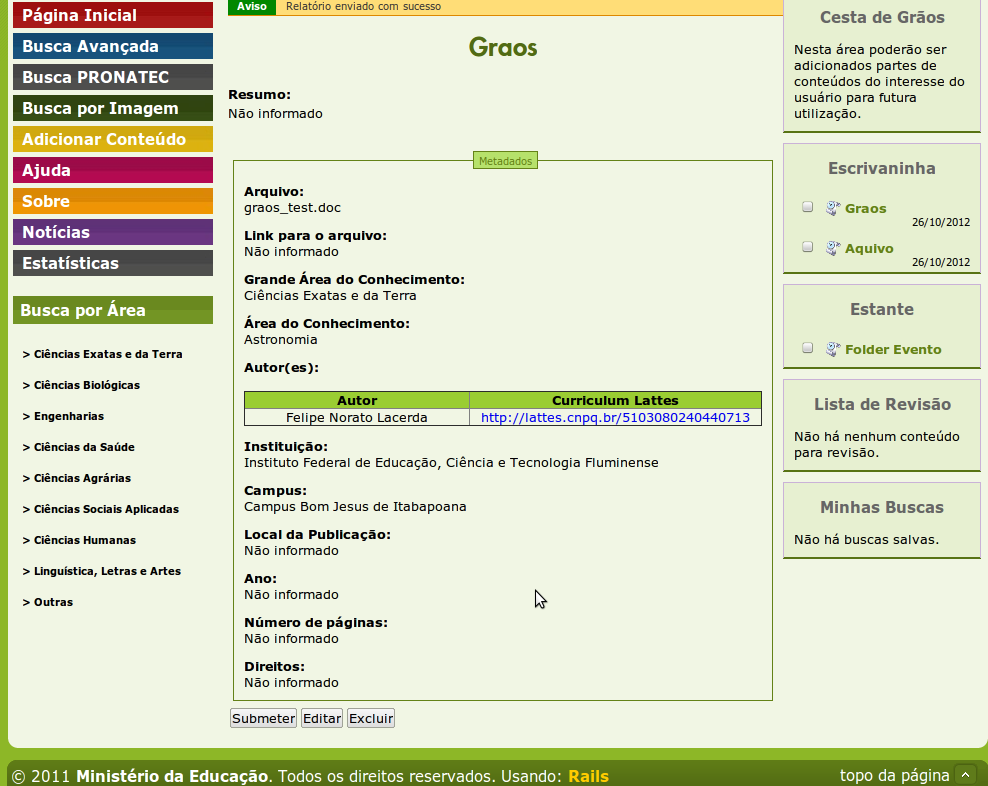
\includegraphics{figuras/submeter}}
    \caption{Pagina de submissão de documentos da Biblioteca Digital}
    \label{submeter}
\end{figure}

\begin{figure}[ht]
    \centering
    \scalebox{0.4}{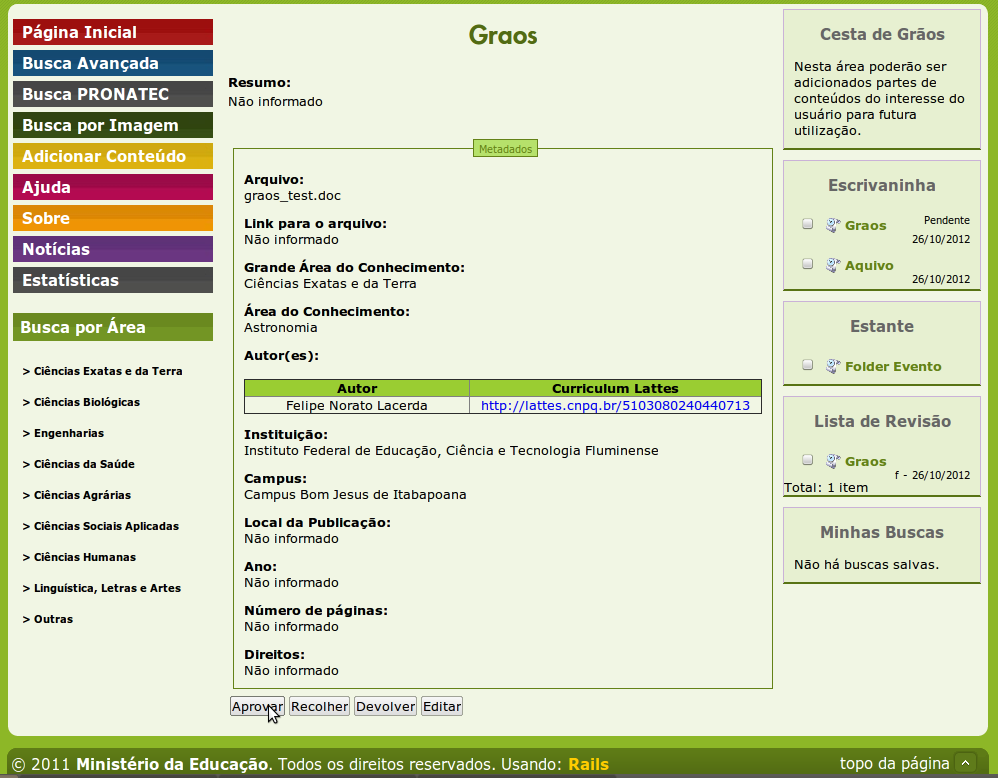
\includegraphics{figuras/aprovar}}
    \caption{Pagina de aprovação de documentos da Biblioteca Digital}
    \label{aprovar}
\end{figure}

\newpage
Nas figuras não é implícito o uso da ferramenta, entretanto, uma vez que essa funcionalidade requer o uso de documentos em formato livre para realização de suas tarefas, é requerido o uso do CloudOoo para converter o arquivo em questão para um padrão livre e posteriormente realizar a funcionalidade de ``granularização''.

\begin{figure}[ht]
    \centering
    \scalebox{0.4}{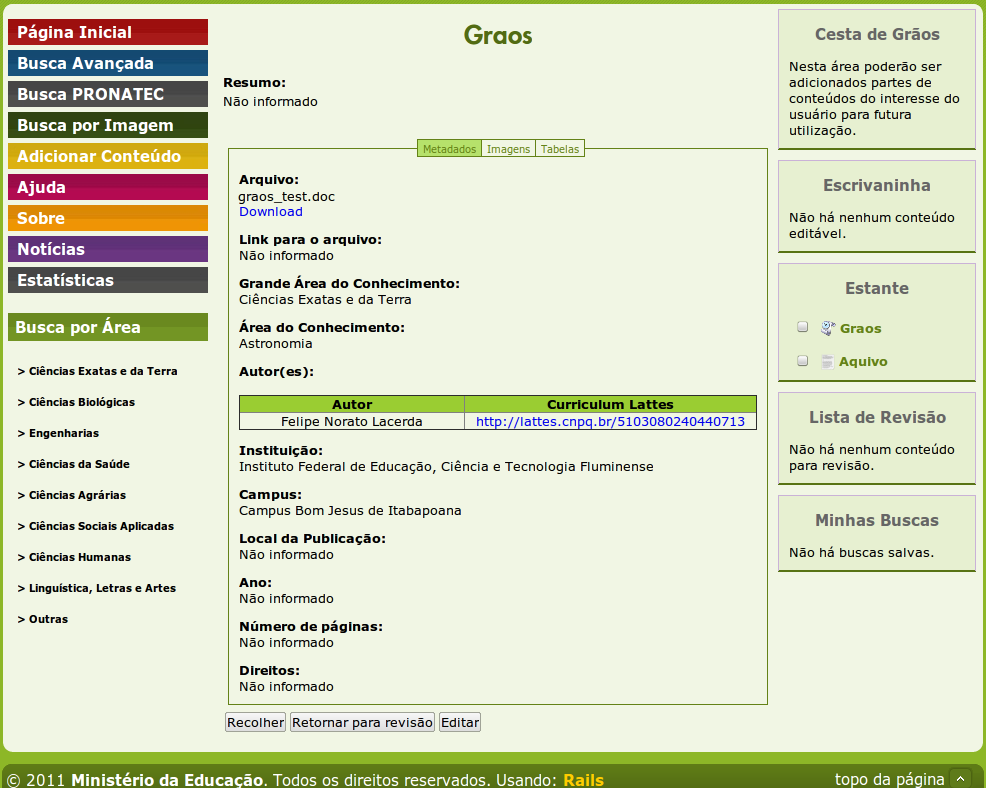
\includegraphics{figuras/metadados}}
    \caption{Pagina de exibição de metadados de documentos da Biblioteca Digital}
    \label{metadados}
\end{figure}

\newpage
Na figura \ref{metadados} há uma demonstração da funcionalidade de extração de metadados, enquanto os grãos encontram-se nas figuras \ref{imagens}:

\begin{figure}[ht]
    \centering
    \scalebox{0.4}{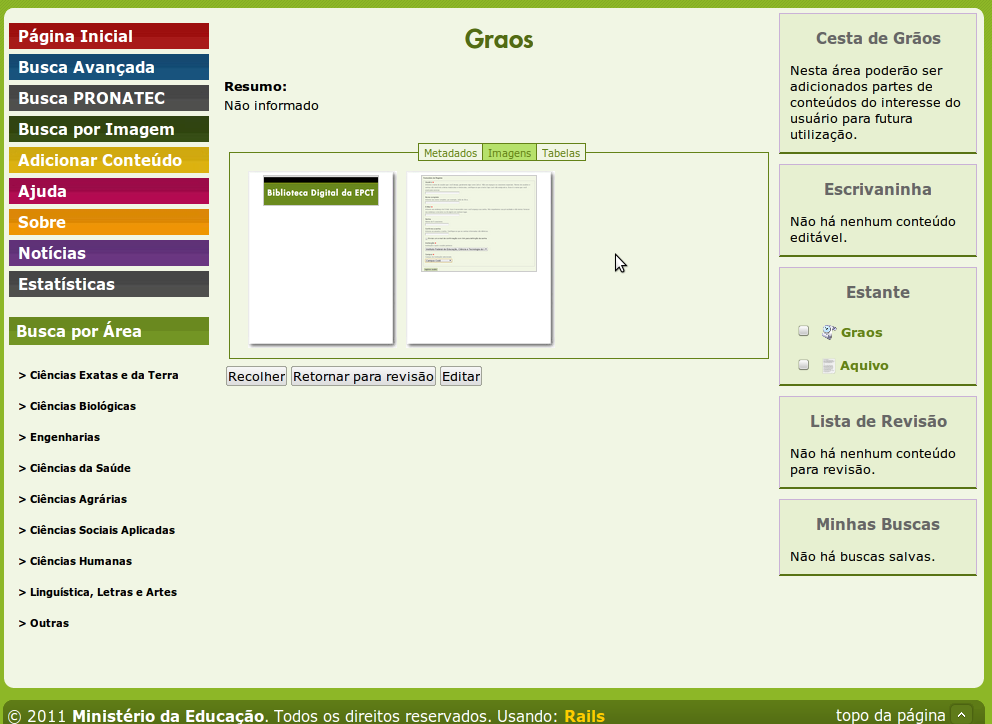
\includegraphics{figuras/imagens}}
    \caption{Pagina de exibição de grãos do tipo imagem de documentos da Biblioteca Digital}
    \label{imagens}
\end{figure}

\newpage
Os grãos extraídos pelo processo de ``granularização'' são separados em imagens(\ref{imagens}) e tabelas, que não existem nesse caso, e dispostos para visualização do usuário.


\newpage
\section{Performance}

Para estabelecer diferença de performance em relação as versões anteriores do CloudOoo foram considerados dois testes.

O primeiro deles realizado em um trabalho anterior, por \citeonline{MONNERAT}, contava 3699 documentos no formato ODT que foram selecionados previamente, entre eles alguns documentos inválidos e outros em formatos desconhecidos. Por ser a conversão mais utilizada, foi decido que neste teste estes documentos seriam convertidos para PDF. 
Este teste foi realizado por meio do uso de um \textit{script}, neles além de prover a conversão também era provido o armazenamento do tempo de cada conversão, bem como o tempo total que todas as conversões levaram em cada versão do CloudOoo.

No resultado do primeiro teste notou-se que o OOOD 2.0 levará mais tempo para realizar a conversão de cada documento,entretanto por ser mais estável levou 10 horas para realizar o teste e apresentou 12 erros, enquanto o OOOD 1.0 apresentou 531 erros e levou 11 horas para realizar o teste.

No segundo teste foram escolhidos arquivos distintos, representado no código \ref{carga}, este teste selecionou 3 diferentes documentos DOC para serem convertidos para ODT; 3 documentos com PDF para serem convertidos para TXT, 1 arquivo de vídeo AVI de aproximadamente 100 MB que seria convertido para THEORA; um arquivo de áudio MP3 de aproximadamente 3 MB para ser convertido para VORBIS; e por fim uma imagem PNG de aproximadamente 30 KB para ser convertida para JPG.

\newpage
{\singlespace
\begin{lstlisting}[caption=\textit{Script} de teste,language=python,label=carga]
from random import randint
from base64 import encodestring, decodestring
from datetime import datetime
from xmlrpclib import ServerProxy
import magic


mime_decoder = magic.Magic(mime=True)

documents = ['ISSCWR6PaperTemplate.doc','SiteLeaderAppWinter2012.doc', 'Estonia.doc']
pdfs = ['Bankruptcies.pdf', 'WIA-IM_tfw_studentguide.pdf', '2012FinancialRpt.pdf']

type_convert_choices = { 0: [documents, "doc", "odt", 'application/vnd.oasis.opendocument.text'],
                  1: ["test.png", "png", "jpg", 'image/jpeg'],
                  2: ["test.mp3", "mp3", "ogg", 'application/ogg'],
                  3: ["test.avi", "avi", "ogv", 'application/ogg'],
                  4: [pdfs, "pdf", "txt", 'text/plain']
                }


proxy = ServerProxy("http://localhost:23000/RPC2")
id = 0
process = []

while True:

  name = 'test'
  file, source_format, destination_format, mime = type_convert_choices[randint(0,4)]
  data = ''
  if type(file) == str: 
    data = open(file).read()
  else:
    name =file[randint(0,2)]
    data =  open(name).read()
  done, mimetype = False, False
  try:
    file = proxy.convertFile(encodestring(data), source_format, destination_format)
    mimetype = mime_decoder.from_buffer(decodestring(file))
    if mimetype == mime:
      done = True
  except:
    done = "Error"
  process.append([id, name, source_format, mime, destination_format, mimetype, done, '\n'])
  id += 1

content = "  id     |          file       |     source         |   dest            |    done          \n" + str(process)
log = open('log.txt', 'w')
log.write(content)
log.close()

\end{lstlisting}
}

O objetivo deste segundo teste era focar nas conversões de arquivos para formatos abertos, que são mais utilizados nos projetos que o CloudOoo atende. 

Além disso a perspectiva era que um menor número de erros aparecesse em função dos inúmeros tratamento utilizados nesta ferramenta. Também haveria um menor número de conversões que a versão anterior em função do tamanho e tempo que arquivos de vídeo, imagem e áudio consomem comparados a documentos.

Para saber se as conversões foram realizadas com sucesso eram verificados os \textit{mimetypes} de cada conversão de acordo com o esperado.

Infelizmente não foi possível a utilização de diversos arquivos aleatoriamente como seria o caso de um ambiente de produção, em função da dificuldade para adquirir estes arquivos por meio da internet que tem sido cada vez mais restrita a downloads.

Neste segundo teste foram utilizados dois computadores diferentes de desenvolvimento, citados em \ref{computadores}, no notebook e no servidor de 4GB de memória.

No notebook a performance foi consideravelmente estável, em 10 horas o CloudOoo realizou 2034 conversões, entre elas 405 conversões foram de DOC para ODT e apenas 3 retornaram erro; 260 foram de PDF para TXT e nenhuma retornou erro; 307 foram de AVI para OGV Theora e nenhuma retornou erro; 384 foram de MP3 para OGG \textit{Vorbis}; e 678 foram de PNG para JPG sem retorno de erro.

Resultando assim em apenas 3 erros em 10 horas.

No servidor, entretanto o resultado foi menos promissor, o teste durou apenas 3 horas em função de um erro de estouro de memória no servidor, que detinha de aproximadamente 3 GB livres para o teste, mas que não se encontrava disposto apenas para o teste uma vez que estava em uso em tempo real. 

Durante essas 3 horas foram realizadas 611 conversões, entre elas 122 conversões foram de DOC para ODT e apenas 1 retornou erro; 77 foram de PDF para TXT e nenhuma retornou erro; 91 foram de AVI para OGV Theora e nenhuma retornou erro; 114 foram de MP3 para OGG Vorbis; e 207 foram de PNG para JPG sem retorno de erro.

De forma positiva o CloudOoo se manteve estável durante essas horas tanto no notebook quanto no servidor, pois mesmo com o estoura de memória no segundo, ele se manteve ativo. Entretanto com os resultados dos teste foi constatado que com as novas funcionalidades adicionadas precisam ser revisadas em função de escalabilidade e uso em tempo real a fim de que não volte a ocorrer estouros de memória entre outros possíveis erros. 

No que respeito aos erros de documentos, dada a falta de variedade, foram todos erros relativos aos documentos PDF com proteção contra conversão.

Na tabela \ref{clooo} mostrando os resultados desses testes:

\begin{table}[!t]
\caption{Comparação entre versões do CloudOoo por meio de testes.}
\label{clooo}
\begin{tabular}{|r|c|c|c|c|p{1.5cm}|p{2cm}|p{1.5cm}|}
\hline
Versões & Documentos & Imagens & Áudio & Vídeo & Total de erros & Total de Conversões & Total de horas \\
\hline
OOOD 1.0 & 3699 & 0 & 0 & 0 & 531 & 3699 & 11 \\
\hline
OOOD 2.0 & 3699 & 0 & 0 & 0 & 12 & 3699 & 10 \\
\hline
CloudOoo & 405+260 & 307 & 384 & 678 & 3 & 2034 & 10 \\
\hline
\end{tabular} 
\end{table}


%\chapter{TECNOLOGIAS SIMILARES}
\thispagestyle{empty}

Este capítulo visa apresentar um estudo a respeito de outras aplicações que se assemelham ao tipo de aplicação que representa o CloudOoo, isto é, aplicações web capazes de realizar conversões de documentos e arquivos de multimídia, e que ainda pudessem manipular informações destes arquivos.

Este estudo foi baseado especialmente em aplicações livres e de código aberto que se encontram disponíveis para uso e colaboração tal como o CloudOoo, dado o pequeno número dessas aplicações também foram estudadas páginas que ofereciam o serviço de conversão on-line.

Entretanto cabe observar que dentre todas aplicações estudados não foi encontrada em nenhuma delas a funcionalidade de extração ou inserção de dados disponíveis no CloudOoo.


\section{inout.io}

O InOut é o serviço web que mais se aproximou de ser uma tecnologia similar ao CloudOoo. Ele foi desenvolvido exclusivamente para lidar com arquivos e suas conversões.

Este serviço é capaz de converter arquivos dos formatos:
\begin{itemize}
    \item{Documentos: PDF, Microsoft Office, OpenDocument, Open Office, Rich Text Format, Comma separated file;}
    \item{Vídeos: MPEG, Quicktime, Microsoft AVI, Windows Media, Microsoft Advanced Streamin, Theora, Flash, Matroska, Blue-Ray tracks,  FLIC, SGI, DL Animation;}
    \item{Áudio: Wave, MP3, MPEG, MIDI, Raw, Windows Media, MPEG 4 audiostream, Dolby Digital, Apple Audio Interchange, Free Lossless audio, Real, Vorbis, Matroska;}
    \item{Imagens: JPEG, GIF, PNG, TIFF, Windows Bitmap, Windows Metafile, Adobe Illustrator vector, Encapsulated post script vector, Post script, Adobe Photoshop, Targa, Zsoft paintbrush, Mac Pict.}
\end{itemize}


Para os formatos de:
\begin{itemize}
    \item{Documentos: PDF, Microsoft World, Open Document Textfile, Open Office Writer, Rich Text Format;}
    \item{Vídeos: MPEG, Flash;}
    \item{Áudio: Wave, MP3.}
    \item{Imagens: JPEG, PNG, GIF.}
\end{itemize}

Através de uma breve analise às listas de conversões é possível notar que embora reconheça muitos padrões, o InOut tem preferência pela saída de arquivos em formatos livres de suas conversões.

Para comunicação entre seu serviço e qualquer aplicação que queira requisitá-lo, existe uma extensa documentação na página \url{https://api.inout.io/InOut-API Documentation.html}, esta documentação é especialmente desenvolvida para outros desenvolvedores.

Nessa documentação é recomendado o uso de RESTful e JSON para realizar a comunicação com o serviço, entretanto a linguagem a se utilizar fica por conta de cliente.

No código \ref{inout} é possível notar um exemplo de uso do InOut em que é requerido todos os padrão de conversão para seu uso através do JSON:

{\singlespace
\begin{lstlisting}[caption=Requisição de perfis do InOut,language=bash,label={inout}]

$ curl -u key:secret https://api.inout.io/profiles/


{"ok": true, "result": [
   {"id": "IMAGE_TO_JPEG"},
   {"id": "IMAGE_TO_PNG"},
   {"id": "IMAGE_TO_GIF"},
   // ...
]}
\end{lstlisting}
}

Demais exemplos de uso do InOut podem ser encontrados na página da documentação citada anteriormente.


\section{ServPDF}

É um serviço web capaz de converter documentos, sejam eles de formatos abertos ou proprietários pela Microsoft.

Ele permite que qualquer documento possa ser convertido para PDF, e que qualquer PDF possa ser convertido em Postscript ou imagens.

É uma ferramenta extremamente simples baseada no Microsoft Office e modificada para atender ao LibreOffice.


\section{Conversões Online}

Fora esses serviços a gama de projetos livres para conversão de arquivos e documentos em geral é extremamente escassa. Existem muitas versões \textit{desktop} e também versões de serviço on-line, neste caso os serviços são hospedados em páginas que ficam disponíveis gratuitamente para usuários.

A desvantagem desses serviços em relação ao CloudOoo é de que normalmente seus arquivos são limitados a um tamanho específico pelos proprietários da página, enquanto para um usuário que hospeda um CloudOoo é possível modificar esse limite de acordo com a máquina qual o mesmo será instalado, podendo este limite ser bem maior, entretanto dependendo do usuário para instalá-lo.

Assim é possível concluir que para um usuário final que não possua conhecimentos avançados de serviços web pode ser bem mais agradável utilizar essas páginas. As próximas subseções mostram alguns exemplos interessantes para seu uso.

\subsection{youconvertit.com}

O You Convert It é uma das páginas disponíveis na web para conversão de documentos, imagens, vídeos e áudio on-line. É uma das páginas mais aconselháveis pois possui o limite de arquivos no tamanha de até 1GB.

\subsection{convertfiles.com}

Assim como o You Convert It, o Convert.Files é capaz de converter desde documentos a arquivos de multimídia, entretanto com um limite bem menor de apenas 150MB por arquivo. Nele existe a vantagem de que o usuário possa mandar os arquivos convertidos para seus celulares ou aparelhos moveis em geral.

\subsection{zamzar.com}

Similar aos exemplos anteriores o Zamzar é capaz de realizar a conversão entre qualquer arquivo, entretanto seu tamanho limite para arquivos é de 100MB e até 5 conversões diárias, apesar disso é um dos serviços mais populares para conversão on-line.


\section{Comparação entres CloudOoo e seus similares}

Na tabela \ref{funsim} com uma comparação entre as funcionalidades dos similares com o próprio CloudOoo:
\begin{table}[!h]
\caption{Comparação entre funcionalidades de ferramentas similares ao CloudOoo.}
\label{funsim}
\begin{tabular}{|r|c|c|c|c|p{1.5cm}|p{1.5cm}|}
\hline
Funcionalidade & CloudOoo & InOut & ServPDF & YouConvertIt & Convert. Files & Zamzar \\
\hline
Servidor de serviços & X & X & X & - & - & - \\
\hline
Converte documentos & X & X & X & X & X & X \\
\hline
Converte Imagens & X & X & - & X & X & X \\
\hline
Converte Áudio & X & X & - & X & X & X \\
\hline
Converte Vídeos & X & X & - & X & X & X \\
\hline
Apresenta metadados & X & - & X & - & - & - \\
\hline
Modifica metadados & X & - & - & - & - & - \\
\hline
\end{tabular} 
\end{table}

Após essa comparação é possível ressaltar a importância do CloudOoo como única ferramenta livre capaz de converter e manipular dados de diferentes tipos de arquivos, além de dispor de uma interface cliente-servidor.

%\chapter{CONCLUSÕES}
\thispagestyle{empty}

\section{Objetivos alcançados}

Neste trabalho foi possível apresentar as contribuições realizadas a ferramenta de conversão e manipulação de arquivos em nuvem, CloudOoo.

Sendo esta apresentação uma simples descrição sobre todos os processos por trás dessas novas funcionalidades, entre elas a conversão e manipulação de áudio e vídeo, e a granularização de documentos PDF.

Além disso este trabalho apresentou detalhadamente a nova estrutura do CloudOoo, descrevendo um pouco sobre o uso desta estrutura dentro do mesmo.

Foram apresentadas também as tecnologias empregadas no CloudOoo, sendo essas aplicações livres e de código aberto, que se encontram disponível para acesso; e ainda outras ferramentas similares a esta aplicação.

Houve também uma breve descrição sobre como instalar e usar esta aplicação como ferramenta de conversão e manipulação de arquivos comuns aos tipos de documentos, imagens, vídeos, áudio e PDF.

Por fim, foi possível afirmar sobre as modificações e melhorias dessas funcionalidades através de um estudo de caso em cima do uso real em ferramentas utilizadas por empresas ao redor do mundo; e também através da realização de testes de escalabilidade comparados entre si e entre testes anteriores.

\section{Trabalhos futuros}

Apesar deste trabalho representar em grande parte a realização de objetivos propostos por um trabalho anterior com a aplicação CloudOoo, nota-se a necessidade de modificações futuras visando a melhoria continua da ferramenta.

Entre essas melhorias, visar maior estabilidade do projeto não só por meio dos testes implementados e seus acréscimos, bem como pela revisão da escrita do projeto em função das novas funcionalidades adquiridas, que se apresentaram poucos estáveis podendo causar problemas com o uso excessivo de memória e do sistema como um todo.

Umas vez que os tipos de arquivos atendidos pelo mesmo foram expandidos também há o interesse de estender funcionalidades mais complexas já aplicadas aos documentos, como por exemplo a ``granularização'' de arquivos de vídeo, que é um processo já disponível e implantado no projeto da Biblioteca Digital.

Além dessas funcionalidades pretende-se que arquivos de multimídia também tenham seu dados tratados.

Por fim é de interesse do projeto que esta ferramenta seja capaz de trabalhar como um serviço RESTful para respostas mais simples e realizadas em diversas aplicações por uma interface JSON.

\bibliography{referencia} % Gera as referências bibliográficas
\end{document} % Fim do TCC
